\documentclass[12pt]{article}   % Précise le type de document, et la taille de la police de caractère
% packages
%----------------------------------------------------------------
% Packages
%----------------------------------------------------------------

\usepackage{natbib} % Pour pouvoir utiliser une bibliographie externe
\usepackage[french]{babel}	% Pour préciser la langue du document
\usepackage[utf8]{inputenc}	% Précise comment le texte est saisi : cela permet de tapper directement les accents
\usepackage[T1]{fontenc}	% Précise la façon dont le document actuel est encodé
\usepackage{setspace}
\usepackage[margin=2.5cm]{geometry} % Précise les marges du document

% Boxes quotation
\usepackage{tcolorbox}

% icones
\usepackage{fontawesome5}

%Sections
%----------------------------------------------------------------
%\usepackage{newclude} % Pour pouvoir utiliser l'étoile après \inculde pour éviter les sauts de page. Ce package a des problême de compatibilité avec la package natbib
%\renewcommand\thesection{} % Pour éviter la numérotation des sections
%----------------------------------------------------------------

%Autres packages et commandes utiles
%----------------------------------------------------------------
\usepackage{amsmath,amsthm,amssymb,amsfonts}	% Pour pouvoir inclure certains symboles et environnements mathématiques
\usepackage{enumerate} % Pour mieux gérer la commande enumerate dans les sections
\usepackage{graphicx}	% Pour inclure des images
\graphicspath{{assets/}}
\usepackage{color}	% Pour inclure du texte en couleur
\usepackage{units}	% Pour pouvoir tapper les unités correctement
\usepackage{pgf,tikz}	% Utilisation du module tikz, qui permet de tracer des belles images
% \usetikzlibrary{arrows} % Quand on exporte une image GeoGebra, on a besoin de préciser cela
\usepackage{hyperref}	% Pour include des liens dans le document
% \usepackage{cprotect}	% Pour pouvoir personaliser la légende des figures
%----------------------------------------------------------------


% variables
\title{Dossier de projet}% N'affecte pas la page titre, mais défini le nom de votre projet
\author{Sofiane MSATFA} % N'affecte pas la page titre, mais défini le nom de l'auteur(e) du projet

%Informations destinées à la page de présentation
%----------------------------------------------------------------
\newcommand{\titre}{Dossier de projet professionnel}
\newcommand{\formation}{Titre professionnel développeur web\\ et web mobile (DWWM)}
\newcommand{\auteur}{Sofiane MSATFA}
\newcommand{\session}{2021-2022}
%----------------------------------------------------------------

% boxe commentaires
\newtcolorbox{commentaire}{
    before=\vspace{0.5cm},
    after=\vspace{0.5cm},
    colframe=blue!40!white,
    colback=blue!8!white
    }

\newcommand{\colored}[1]{{\color{red!55!orange}#1}}

\begin{document}

% page de couverture
\thispagestyle{empty}	% Pour éviter d'avoir un en-tête et un pied de page sur la page couverture


\includegraphics[width=8cm]{logo.jpg}	% Pour inclure le logo (on précise la largeur de l'image)

\vspace{4cm}	% Espacement vertical

\begin{center}	% On centre le texte
    {\huge \bf \titre}\\	% \huge fait que le texte est gros, \bf fait que le texte est gras
    \vspace{4cm}
    {\large \formation}\\
    \vspace{4cm}
    réalisé par \\ \auteur \\
    \vfill	% On va jusqu'au bas de la page avant de mettre le texte ci-dessous
    \session
    \pagebreak
\end{center}
    % Inclut le code contenu dans un fichier comme s'il était entré ici

% table des matières
\tableofcontents

% sections
% Le package newclude mis en commentaire permet d'introduire une * pour éviter le saut de page entre les section
\section{Introduction}

Dans le cadre de ma formation développeur web et web mobile, j’ai eu la chance d’assister Mr. Vincent VAURETTE qui est en charge de la cellule de transition numérique de la Fédération Française de Volley-Ball (FFVB).\\
Le but de son travail est de développer des outils qui facilitent la gestion de tout ce qui est en lien avec le monde du volley-ball, et de redonner un coup de jeune à l’intranet de la fédération.\\
Durant trois mois, j’ai eu la responsabilité de la transition numérique de l’interface de désignation des arbitres.

\vspace{1cm}


\includegraphics{logo.jpg}

La Fédération Française de Volley-Ball est une association créée en 1936 qui constitue l’instance dirigeante du volley-ball en France. 
Plusieurs centaines de matchs se déroulent par week-end, et la désignation des arbitres les concernant est entrêmement chronophage.


\begin{commentaire}
    Le site actuel de la fédération date de 2009 et manque d’ergonomie. Celui-ci demande plusieurs click pour effectuer une seule désignation et ne permet pas d’afficher toutes les informations nécessaires pour celles-ci. Les gestionnaires sont alors contraints de passer par un tableur externe pour procéder aux désignations, puis ensuite de rentrer manuellement celles-ci pour chaque match.
\end{commentaire}


L’objectif principal qui m’a été confié a été la création d’un outil permettant d’automatiser ces désignations. Celui-ci devait pouvoir associer un ou plusieurs arbitres habilités et disponibles à chaque match d’une période donnée, tout en laissant le choix de leur modification.
\subsection{Cahier des charges}
% Dans ce document, je fais référence au livre de Paul Ver Eecke \cite{VerEecke1960Archimede} et à celui de Sherman Stein \cite{stein1999archimedes} et \cite{minda2008triangles}.

\subsubsection{Objectifs}
\textit{Quels sont les objectifs demandés ?}\\

\begin{itemize}
    \item L’objectif principal est l’automatisation des désignations des arbitres pour une période donnée. Il faut que cet algorithme puisse proposer un arbitre habilité et disponible pour chaque match de la période voulue.
    \item Un autre objectif essentiel est la mise en place d’une matrice des distances entre chaque arbitre et chaque club, qui pourra servir à faciliter la désignation des arbitres pour les gestionnaires.
    \item Enfin, il faut également améliorer l’interface graphique et ajouter quelques fonctionnalités.
\end{itemize}

\vspace{1cm}

\textit{Quelles sont les fonctionnalités à ajouter à l’interface ?}\\

\begin{itemize}
    \item Il faut que l’interface affiche tous les matchs à venir de la saison sous forme de tableau, qu’on pourra également trier par poule si voulu. Pour le confort des utilisateurs, Le tri par poule doit se faire sous forme de SELECT avec la possibilité de rechercher une valeur dans celui-ci.
    \item Le tri des matchs par colonne doit être possible et une pagination doit être mise en place.
    \item (Optionnel) Une barre de recherche doit également être disponible pour trouver une donnée précise dans ce tableau.
    \item Il faut pouvoir désigner les arbitres directement depuis cette interface, en affichant un SELECT avec une liste de tous les arbitres disponibles. Cette liste d’arbitres doit afficher plusieurs informations essentielles les concernant : le numéro de licence, le niveau, le grade, et la distance les séparant du gymnase du match. Les arbitres doivent également être triés par état de disponibilité pour le match sélectionné, avec un code couleur différent pour chacun.
    \item La désignation doit se faire de façon automatique au changement du SELECT pour éviter de perdre les sélections en cas d’oubli.
    \item L'interface doit également permettre de lancer l’algorithme d’automatisation des désignations en permettant de choisir une période voulue et de lancer les désignations via un bouton.
\end{itemize}

\newpage

\textit{Précisions concernant l'automatisation des désignations ?}\\

\begin{itemize}
    \item Il faut pouvoir distinguer les matchs pour lesquelles deux arbitres sont nécessaires, et proposer le bon nombre d’arbitres à chaque fois. 
    \item Il ne faut proposer que des arbitres qui sont habilités à arbitrer, et disponibles le jour du match : c’est à dire qui n’ont pas précisé d’indisponibilité, et qui ne sont pas déjà désignés sur un autre match. 
    \item Prendre en compte les exceptions : les arbitres ne peuvent pas arbitrer un match joué par leur club, et les matchs du club à qui ils ont donné leurs points d’arbitrage.
    \item La distance séparant les arbitres du gymnase doit aussi être prise en compte, mais être flexible pour éviter les désignations répétitives des mêmes arbitres pour les mêmes gymnases.
    \item L’algorithme doit proposer des arbitres pour chaque match de la période, mais également permettre le changement manuel de ceux-ci directement sur l’interface. De plus, la validation des désignations automatiques, contrairement aux désignations manuelles, devra se faire grâce à un bouton de confirmation.
    \item Certains matchs sont de type ‘tournois’ et se déroulent donc au même endroit : l’algorithme doit proposer le même arbitre pour chaque paquet de trois matchs de la même poule du même tournois.
\end{itemize}


\subsubsection{Contraintes techniques}

Les technologies utilisées sont :\\

\begin{itemize}
    \item Bootstrap 4.6 (une autre version peut cependant être utilisée)
    \item Javascript / JQuery 3.6
    \item PHP 8 (aucun framework)
    \item MySQL 8.0
\end{itemize}

\section{Mise en place du projet}
\vspace{1cm}

Afin de répondre à ces objectifs, il m’a fallu mettre en place un plan d’action en prenant compte les technologies utilisées pour ce projet.\\
Mon travail devait pouvoir être maintenu facilement par mon tuteur, et pour ce faire la documentation et l’organisation des fichiers étaient primordiales.

\begin{commentaire}
    Une documentation complète a été réalisée en fin de projet pour apporter une précision supplémentaire aux commentaires écrits avec le standard d'écriture PHP Docs, permettant ainsi de faciliter la compréhension et la reprise du projet par mon tuteur.
\end{commentaire}

J'ai décidé de travailler en Programmation Orientée Objet (POO) pour faciliter la réutilisation des composants.\\
J’ai donc pensé à organiser mes fichiers par entité qui compose ce projet : chaque classe concernant une entité se trouve dans un dossier différent des autres et permet ainsi de facilement s’y retrouver dans les fichiers.

\begin{figure}[!h]
    \centering
    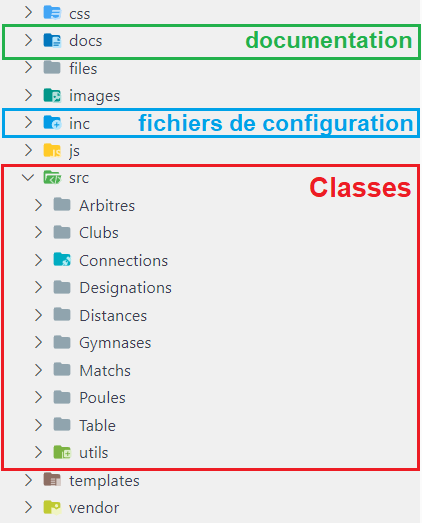
\includegraphics[width=0.5\linewidth]{architecture.png}
    \caption{Arborescence des dossiers du projet}
\end{figure}

\pagebreak

Pour effectuer cette séparation des fichiers sans compliquer l’utilisation des classes, j’ai adopté le concept de namespace et utilisé le gestionnaire de dépendances Composer pour ce projet.

\begin{commentaire}
    Composer est un gestionnaire de dépendances pour PHP. Il permet de réduire l’importation de fichiers en automatisant cette tâche.
\end{commentaire}

\vspace{2cm}

\faIcon{arrow-alt-circle-right} Je commencerai par expliquer les méthodes utilisées pour récupérer les données nécessaires à ce projet, puis j’exposerai les modifications apportées à l’interface graphique et enfin je parlerai en profondeur de l’algorithme d’automatisation des désignations. 

\section{Récupération des données}
\vspace{1cm}

Par manque d’accès à la base de données fédérale, la première étape consistait à récupérer les données nécessaires à la mise en place des outils.\\
Après une analyse complète des informations nécessaires au projet, j’en suis arrivé au modèle de données UML suivant :

\begin{figure}[!h]
    \centering
    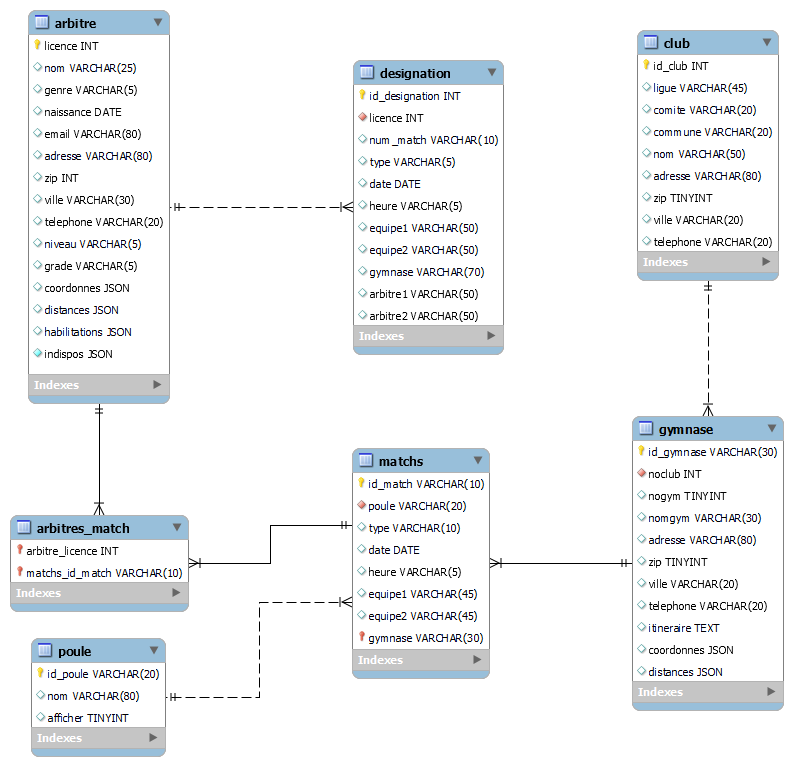
\includegraphics[width=\linewidth, height=15cm]{UML_DPP.png}
    \caption{Modèle de données UML effectué avec MySQL Workbench}
\end{figure}

\vspace{0.5cm}

Certaines données étaient disponibles au format csv (Excel), et d’autres demandaient à être récupérées sur l’intranet actuel de la fédération. Il m’a donc fallu extraire ces dernières via Web Scrapping pour ensuite les insérer dans ma base de données.
\subsection{Configuration}
\vspace{1cm}

Dans un premier temps, afin de faciliter la configuration de l’accès à la base de données lors de la mise en production, j’ai mis en place un fichier de configuration général \colored{globals.php}.\\
Ce fichier contenait un panel de variables de configuration différentes en fonction de l’environnement (développement ou production).
\subsection{Récupération via scraping}
\vspace{1cm}

Pour avoir accès aux données indisponibles sous format Excel, il m’a fallut utiliser \colored{libcurl} pour récupérer le contenu du site actuel de la fédération.\\

Il s’agit d’une bibliothèque permettant de se connecter et de communiquer avec différents types de serveurs, et ce, avec différents types de protocoles. \\

Celle-ci m’a donc permis via le protocole HTTP de me connecter au site de la fédération avec des identifiants fournis par mon tuteur, de stocker les paramètres de connexion, et d’accéder au contenu HTML complet du site sous forme de chaîne de caractères.\\

Il m’a alors fallu analyser cette chaîne de caractères pour en tirer les informations qui m’intéressent, puis insérer celles-ci dans la base de données.

\subsubsection{Connexion}
\vspace{1cm}

Le langage PHP permet le support de \colored{libcurl} via l’extension `CURL` (Client URL Request Library), qui est disponible sous forme d’objet.

Celui-ci possède trois modules en fonction de l’utilisation voulue : un gestionnaire simple, un gestionnaire multiple et un gestionnaire de partage. Les ressources liées à ces gestionnaires sont respectivement \colored{CurlHandle}, \colored{CurlMultiHandle} et \colored{CurlShareHandle} depuis la version PHP8 \\

Dans le cadre de ma problématique, l’utilisation du gestionnaire simple était suffisante. Cependant, une connexion au site de la fédération était nécessaire avant toute récupération de contenu sur celui-ci. \\

Pour faire cela sans multiplier inutilement les connexion pour mes différentes requêtes, j’ai choisi de créer une classe permettant de configurer les paramètres de connexion et de les stocker dans l’objet \colored{CurlHandle} qui me permettait ensuite d’effectuer mes requêtes.

Une fois la connexion effectuée, un cookie était également généré par la librairie pour permettre l’authentification des prochaines requêtes.

\newpage

\begin{figure}[!h]
    \centering
    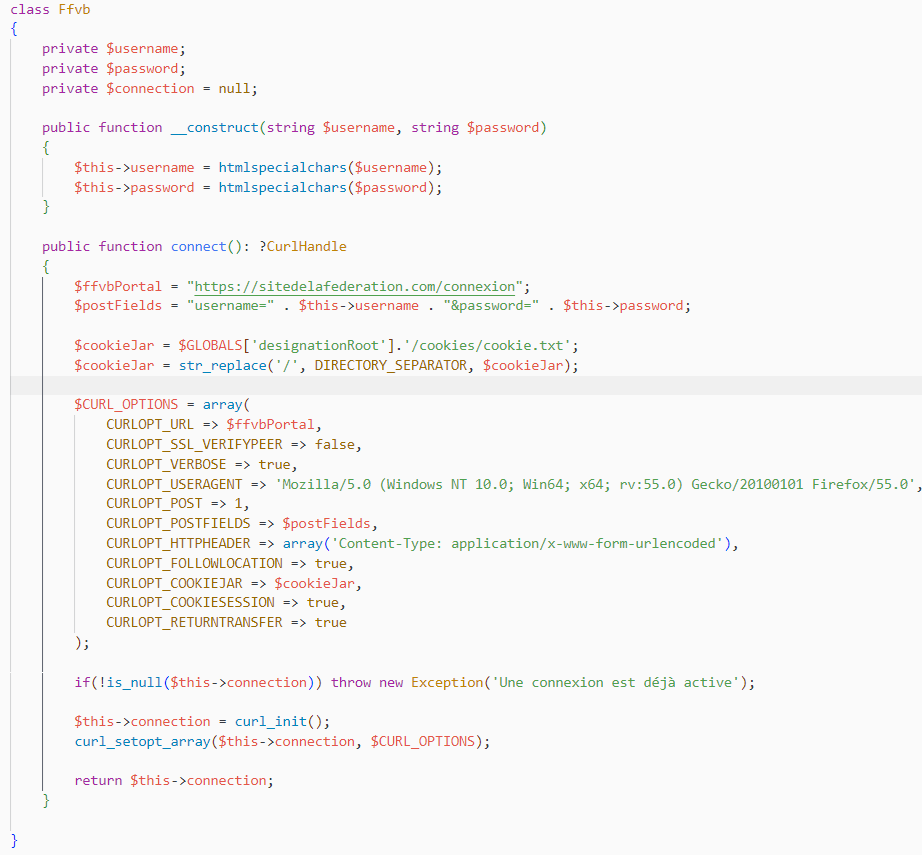
\includegraphics[width=\linewidth]{curl_code.png}
    \caption{Composant de paramétrage d'une connexion au site de la fédération}
\end{figure}

\newpage

\subsubsection{Analyse}
\vspace{1cm}

Les différents outils mis en place pour la récupération des données sur le site de la fédération prennent en paramètre le \colored{CurlHandle} de la connexion configuré précédemment pour effectuer leurs requêtes.\\

Après avoir défini le chemin vers les cookies de ma connexion, il m’a suffit d’envoyer une requête HTTP à la bonne URL pour y récupérer le contenu brut sous forme de chaîne de caractères.

\begin{figure}[!h]
    \centering
    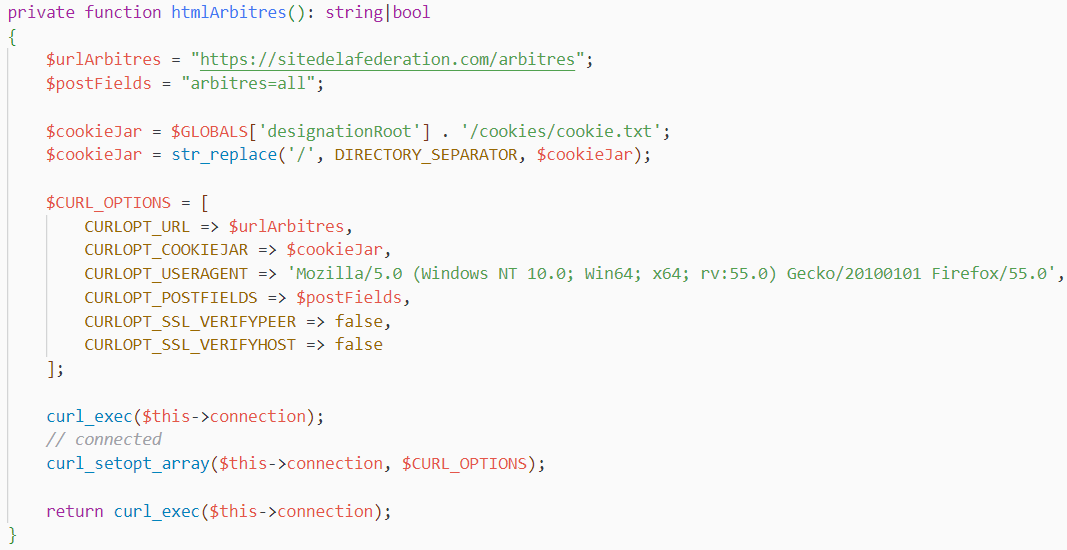
\includegraphics[width=\linewidth]{html_code.png}
    \caption{Méthode de récupération du contenu d'une page de l'intranet}
\end{figure}

\vspace{0.5cm}

Le contenu étant sous forme de chaîne de caractères, le principal problème était de récupérer seulement les informations utiles depuis cette String. Les données sont sous forme de tableaux, et le ciblage de ceux-ci est impossible dans cet état.

Heureusement, PHP possède nativement l’objet \colored{DOMDocument} qui permet d’analyser une chaîne de caractères afin de récupérer les éléments voulus comme nous l’aurions fait en JavaScript. 
En effet, cet objet possède plusieurs méthodes similaires et permettait donc de répondre à mon problème.\\

Cette étape d’analyse étant nécessaire pour toutes mes classes de récupération de données via \colored{CURL} , il m’a semblé logique de créer un objet spécialement conçu pour ça.

De plus, les données à récupérer étant pour la plupart sous forme de tableaux, j’ai également pensé à créer une méthode permettant de récupérer le détails des tableaux contenus dans une chaîne de caractères à partir de l’instance \colored{DOMDocument} liée à celle-ci.

\newpage

\begin{figure}[!h]
    \centering
    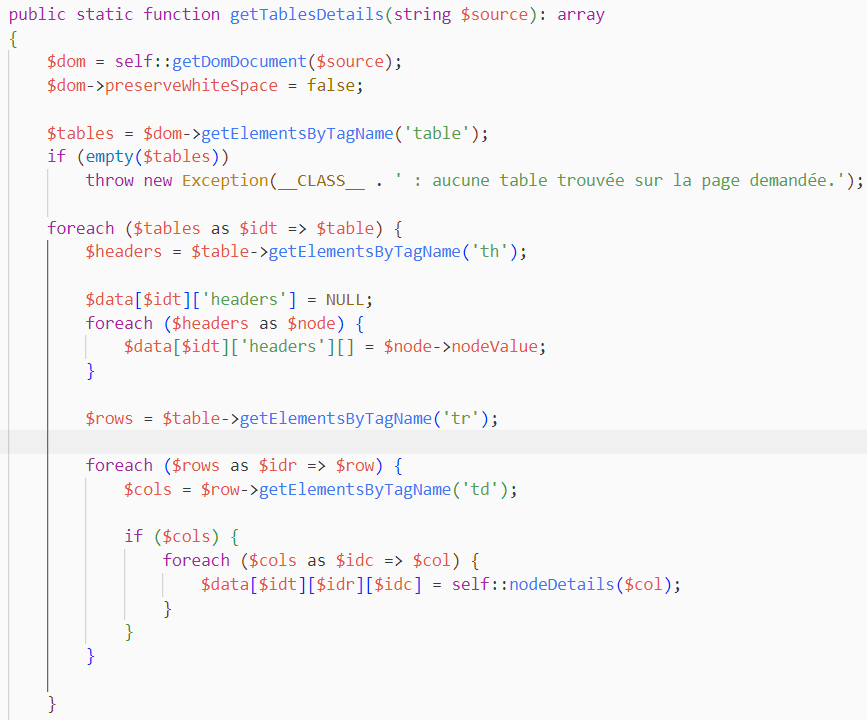
\includegraphics[width=\linewidth]{details_code.png}
    \caption{Méthode d'analyse du contenu d'une page HTML}
\end{figure}

\vspace{0.5cm}

Les détails des colonnes sont récupérés grâce à la méthode \colored{nodeDetails()} qui permet de scanner chaque colonne en récupérant le texte et les attributs si disponibles. Cette méthode effectue ce travail de façon dynamique pour chaque sous-nœud d’une colonne en se rappelant elle-même.

\newpage

\begin{figure}[!h]
    \centering
    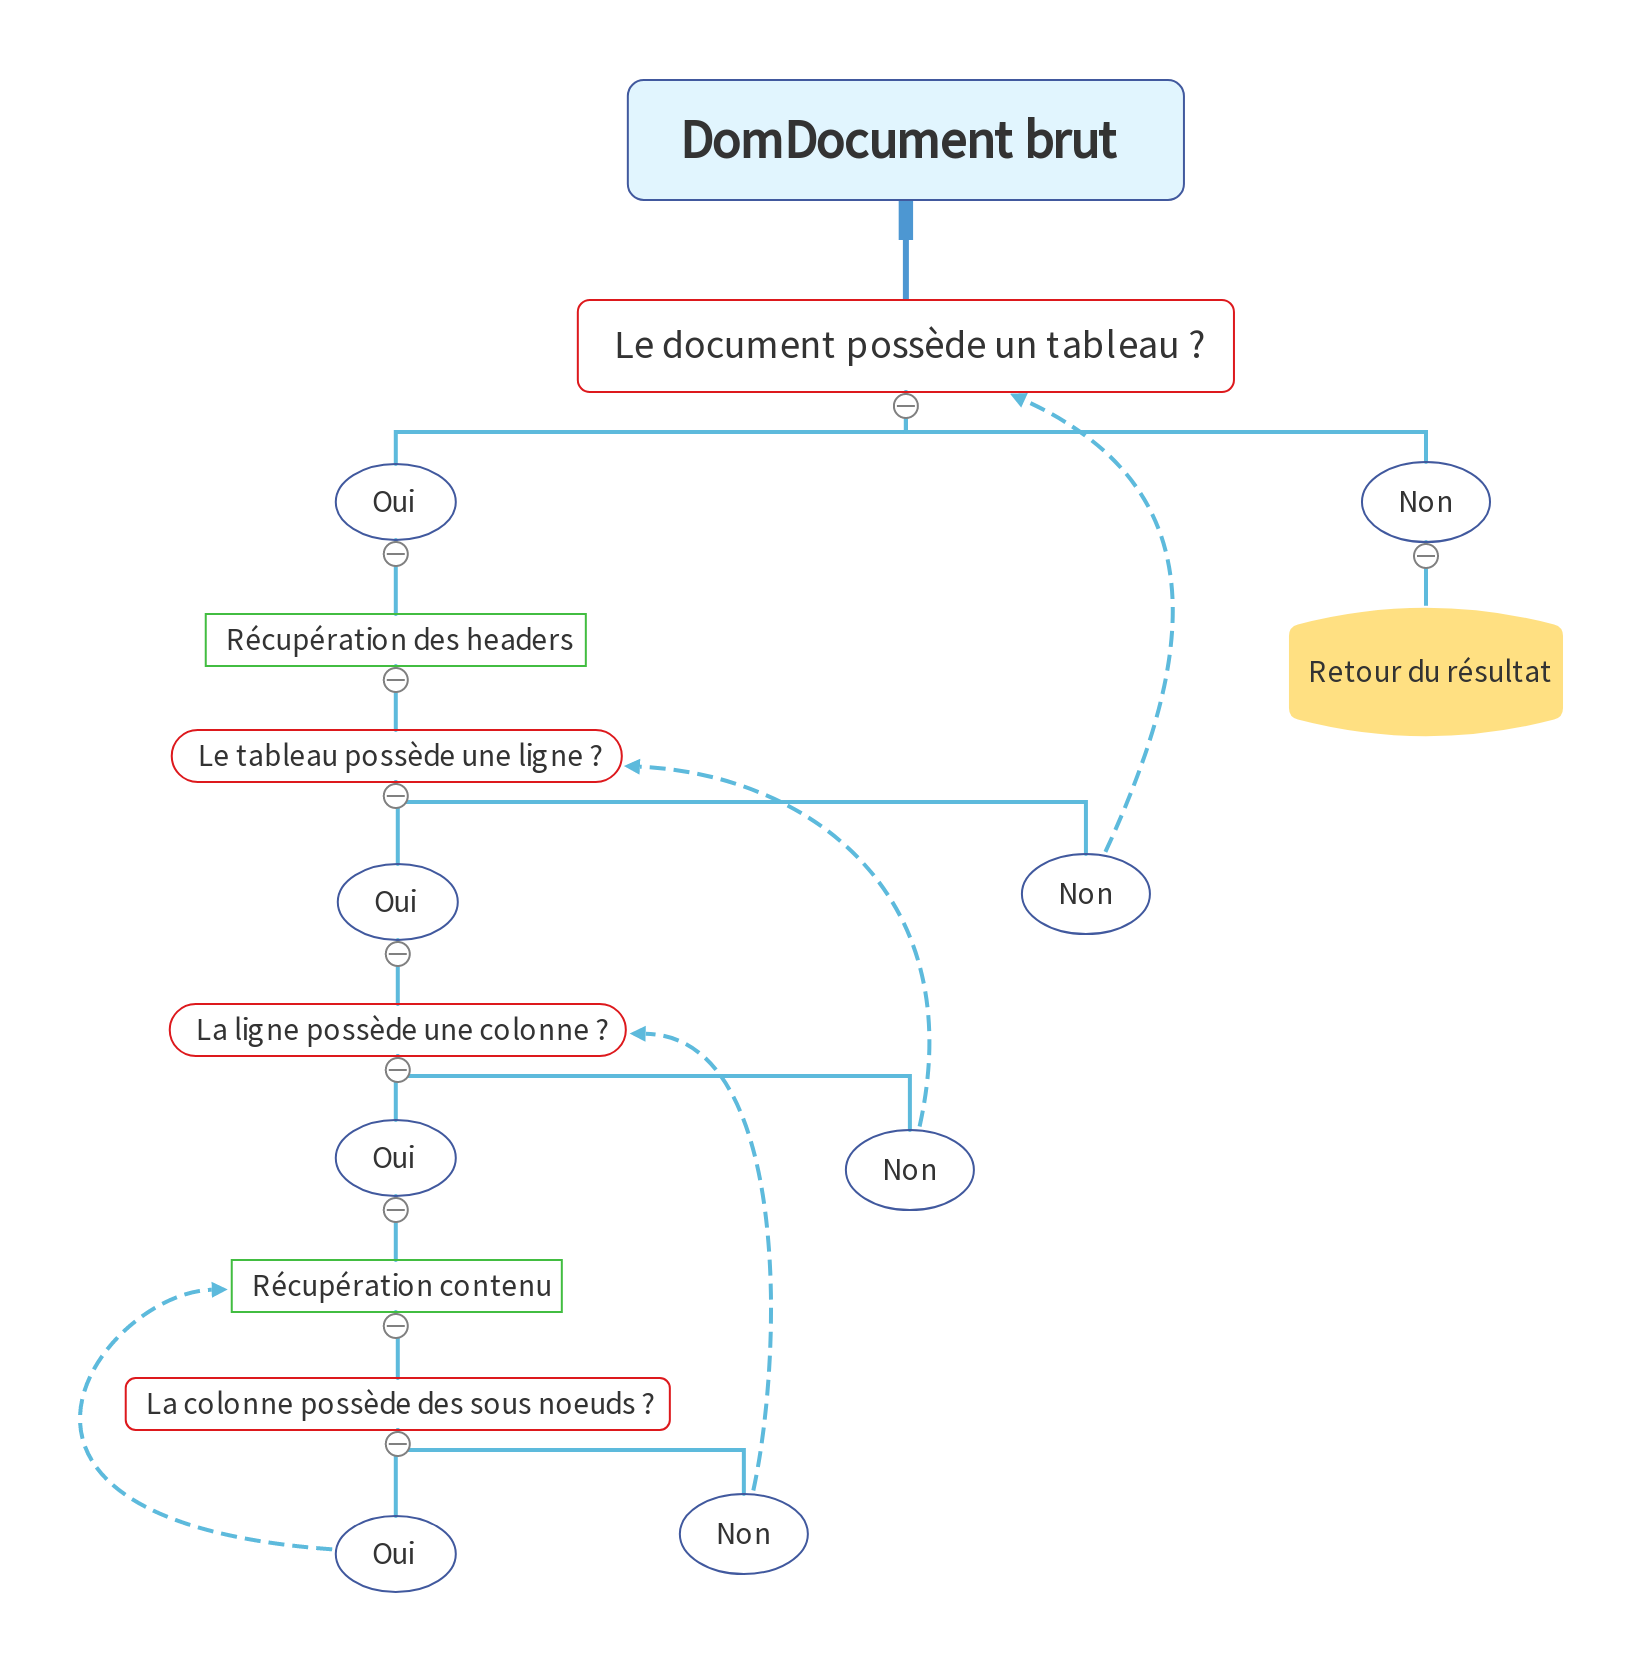
\includegraphics[width=\linewidth]{table_details.png}
    \caption{Logique suivie par la méthode d'analyse du contenu d'une page}
\end{figure}

\vspace{0.5cm}

Une fois ces objets et méthodes mis en place, la récupération et l’analyse des pages intéressantes du site de la fédération étaient beaucoup plus simples. 

J’ai donc ensuite créé une méthode propre à chacune de mes classes permettant de cibler et nettoyer les données renvoyées par les méthodes précédentes. Celles-ci ciblent les attributs et textes renvoyés par la méthode \colored{getTablesDetails()} pour afficher un tableau contenant l’essentiel des données voulues.

\newpage

\subsubsection{Insertion}
\vspace{1cm}

Pour stocker ces données dans la base de données, j’ai d’abord récupéré le nom des tables et colonnes concernées dans le fichier config.json (voir configuration), puis j’ai réutilisé ma classe Database pour effectuer une connexion avec celle-ci.

\begin{figure}[!h]
    \centering
    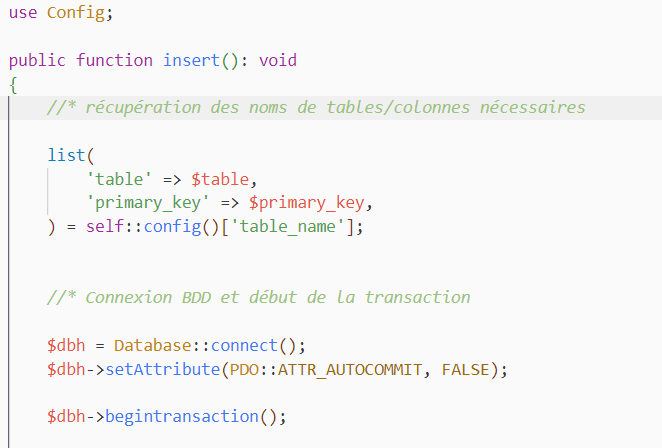
\includegraphics{insert1_code.png}
    \caption{Initialisation de l'insertion des données}
\end{figure}

Pour effectuer cette tâche de façon rapide et sécurisée, j’ai préféré utiliser des transactions et des requêtes préparées lors de la création des données. 
Les requêtes préparées permettent d’augmenter les performances en minimisant les allers-retours avec la base de données. 
Quant à elles, les transactions permettent d’éviter la perte de données dans le cas où certaines des requêtes ne passeraient pas.

De plus, l’objet PDO donne la possibilité de nettoyer les données lors de l’exécution en utilisant des variables nommées ou anonymes dans la requête, permettant ainsi d’éviter les \textbf{injections SQL}.

\begin{commentaire}
    Les injections SQL sont des méthodes permettant de détourner les requêtes SQL en injectant des bouts de codes malicieux.
\end{commentaire}

\begin{figure}[!h]
    \centering
    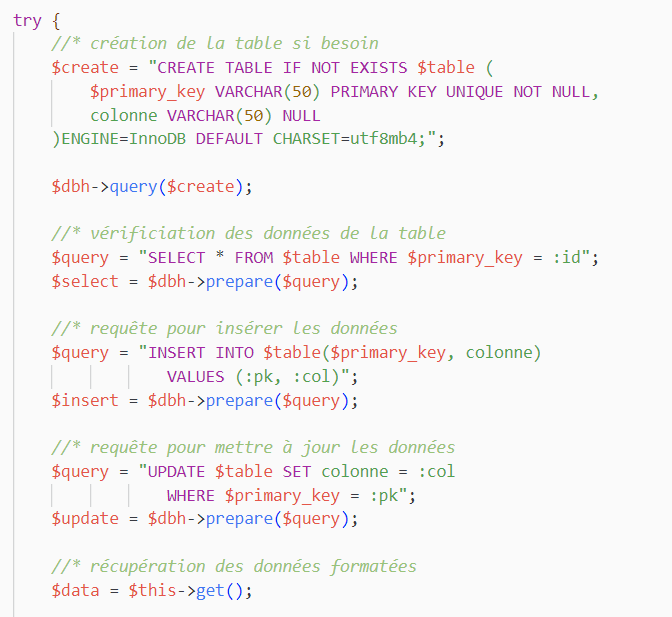
\includegraphics[width=12cm]{insert2_code.png}
    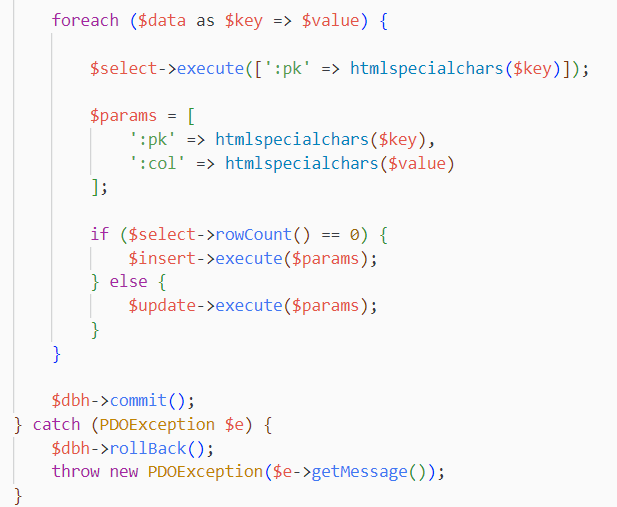
\includegraphics[width=12cm, height=10cm]{insert3_code.png}
    \caption{Insertion de toutes les données de façon sécurisée}
\end{figure}

\newpage

La logique de la méthode \colored{insert()} est de vérifier si les informations à insérer existent déjà dans la base de données, de les mettre à jour dans ce cas, et de les insérer dans le cas contraire. Ceci évite alors les erreurs SQL dues à la multiplicité des clés primaires.\\

Cette étape d’insertion des données m’a également permis d’uniformiser les données récupérées sur différents points d’entrées du site de la fédération, comme par exemples les matchs régionaux et nationaux.\\

En effet, les matchs régionaux et nationaux se trouvent sur deux parties différentes du site officiel et la récupération des informations liées à ceux-ci via scraping ne renvoient pas exactement le même type de données. Cette étape d’insertion était donc l’occasion d’uniformiser les informations qui seraient disponibles pour les uns mais pas les autres, en définissant des valeurs par défaut quand nécessaire.
\subsection{Récupération via fichiers Excel}
\vspace{1cm}

Heureusement, certaines données étaient disponibles directement sous format Excel. Le traitement de celles-ci était donc beaucoup plus facile que précédemment.

Il m’a simplement fallu placer les fichiers Excel dans un dossier, et définir le bon chemin d’accès à ceux-ci dans mon script. \\

Ensuite en ouvrant un stream du fichier grâce à la fonction \colored{file} , qui renvoie un tableau du contenu, j’ai pu analyser celui-ci grâce à une combinaison des fonctions \colored{array\_map} et \colored{str\_getcsv} pour en tirer un tableau multidimensionnel des lignes du fichier Excel.

Chaque ligne du fichier Excel était sous forme de tableau de chaîne de caractères qu’il fallait ensuite séparer par colonnes, en utilisant le séparateur utilisé dans le fichier.

\begin{figure}[!h]
    \centering
    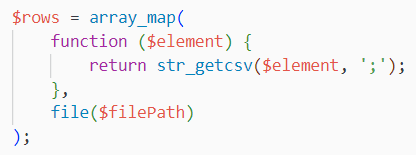
\includegraphics{excel1.png}
    \caption{Parging du fichier Excel}
\end{figure}


Puis en itérant dans chaque ligne de mon fichier, j’ai pu insérer les données voulues dans la base de données en tenant compte de l’encodage des caractères qu’il fallait convertir pour être en accord avec l’encodage de la base de données.


\begin{commentaire}
    Les fichiers Excel sont encodés en \colored{Windows-1252} (ou \colored{CP1252}) et doivent donc être convertis en \colored{UTF-8} pour prendre en compte les caractères accentués par exemple.
\end{commentaire}


\begin{figure}[!h]
    \centering
    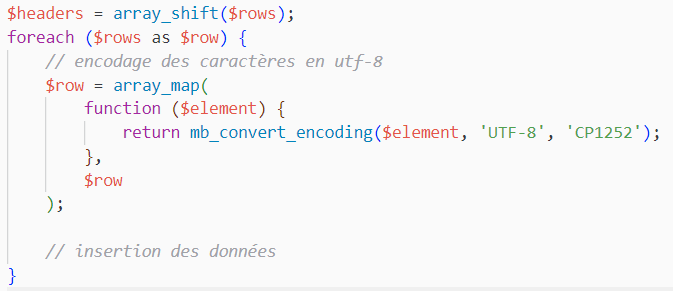
\includegraphics[height=5cm]{excel2.png}
    \caption{Encodage des caractères du fichier}
\end{figure}

\newpage

\subsubsection{Insertion}
\vspace{1cm}

Après avoir récupéré les noms des tables et des colonnes dans \colored{config.json}, j’ai encore une fois utilisé des requêtes préparées et des transactions par soucis de performance et de sécurité.

Les valeurs étant déjà encodées et donc prêtes à être ajoutées à la base de données, j’ai suivi le même principe que pour l’insertion des données via \colored{CURL} , c’est à dire :

\begin{enumerate}
    \item Vérifier si la ligne existe déjà
    \item Si elle existe, alors mettre à jour les données (`UPDATE table`)
    \item Si elle n’existe pas, insérer les données (`INSERT INTO table`)
\end{enumerate}
\subsection{Distances}
\vspace{1cm}

Une tâche nécessaire à la mise en place de l’algorithme d’automatisation des désignations d’arbitres était de pouvoir quantifier la distance séparant les arbitres des gymnases. Cette donnée devait servir de critère lors de la sélection automatique, mais devait également être disponible directement sur l’interface. 

Les distances entre les arbitres et les gymnases devaient donc être stockées en base de données sous forme de matrice pour permettre de récupérer facilement une distance entre le domicile d’un arbitre et l’adresse d’un gymnase.
Face à ce problème, j’ai pensé à deux façon différentes de procéder : 
\begin{itemize}
    \item En créant une table unique associant une ligne par arbitre et une colonne par gymnase, l’intersection de chaque définissant une distance
    \item En stockant la matrice au format JSON dans une colonne de la table des arbitres, qui associe pour chaque arbitre l’id de chaque gymnase et sa distance avec celui-ci, puis effectue de façon symétrique cette étape dans la table des gymnases.
\end{itemize}

Le nombre d’arbitres et de gymnases étant évolutif et de l’ordre de plusieurs centaines, la deuxième option me paraissait plus facile à maintenir et à mettre en place.

\subsubsection{Coordonnées géographiques}
\vspace{1cm}

La première étape était de réfléchir à un moyen de récupérer les distances entre deux adresses. Pour ça deux méthodes s’offraient à moi :
\begin{itemize}
    \item La première était d’utiliser l’API Google Geocoding pour tous les arbitres et les gymnases. Cette API permet de récupérer les coordonnées GPS d’une adresse (longitude et latitude), ce qui pouvait me permettre de calculer la distance à vol d’oiseau séparant chaque arbitre et chaque gymnase grâce à une formule mathématique (Loi des cosinus).
    \item La deuxième méthode était d’utiliser l’API Google Matrix. Cette API permet de récupérer directement la matrice des distances entre une adresse de départ et plusieurs adresses d’arrivée.
\end{itemize}

Pour commencer, j’ai opté pour l’utilisation de la première méthode car celle-ci me permettait de réduire le nombre total de requêtes envoyées à Google.\\ 

En effet, cette méthode ne demandait qu’une requête par arbitre et par gymnase, ce qui équivalait pour $n$  arbitres et $m$ gymnases à un total de $n + m$  requêtes. La deuxième méthode demandait quant à elle un total de $n * m$ requêtes. Google n’autorise cependant qu’un nombre limité de requêtes gratuites par jour que je voulait éviter de dépasser.\\

La recherche de la formule mathématique permettant de calculer une distance entre deux points à partir de leurs coordonnées GPS a été faite sur des sites anglophones à cause du manque d’informations sur les sites francophones.

\newpage 

\begin{figure}
    \centering
    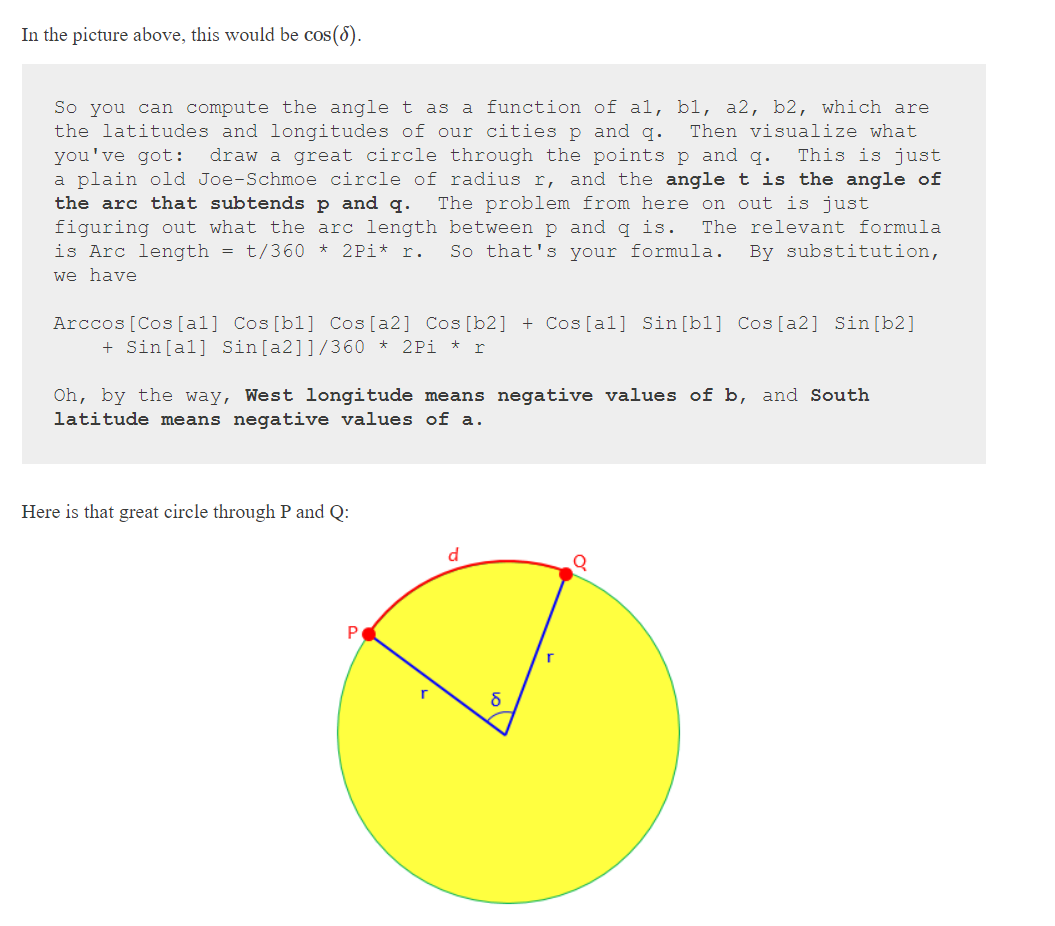
\includegraphics[width=\linewidth]{site_anglais.png}
    \caption{Article anglophone donnant une formulume pour calculer une distance à partir des coordonnées GPS}
\end{figure}

\begin{commentaire}
    Traduction : On peut calculer l’angle delta comme une fonction de paramètres a1, b1, a2 et b2 représentants respectivement les latitudes et longitudes des points P et Q. 
    Pour visualiser ce qu’on a : on dessine un cercle passant par nos points P et Q.
    Il s’agit simplement d’un cercle de rayon r, l’angle delta étant l’angle de l’arc qui relie les points P et Q. Le problème ici est de savoir quel est la distance de l’arc entre les points P et Q. La formule pertinente est : $d = \delta/360 * 2\pi * r$
\end{commentaire}

Pour effectuer le calcul de distance à partir de cette formule, j’ai mise en place un Trait possédant les méthodes nécessaires à la conversion de ces coordonnées en distances.

\begin{figure}[!h]
    \centering
    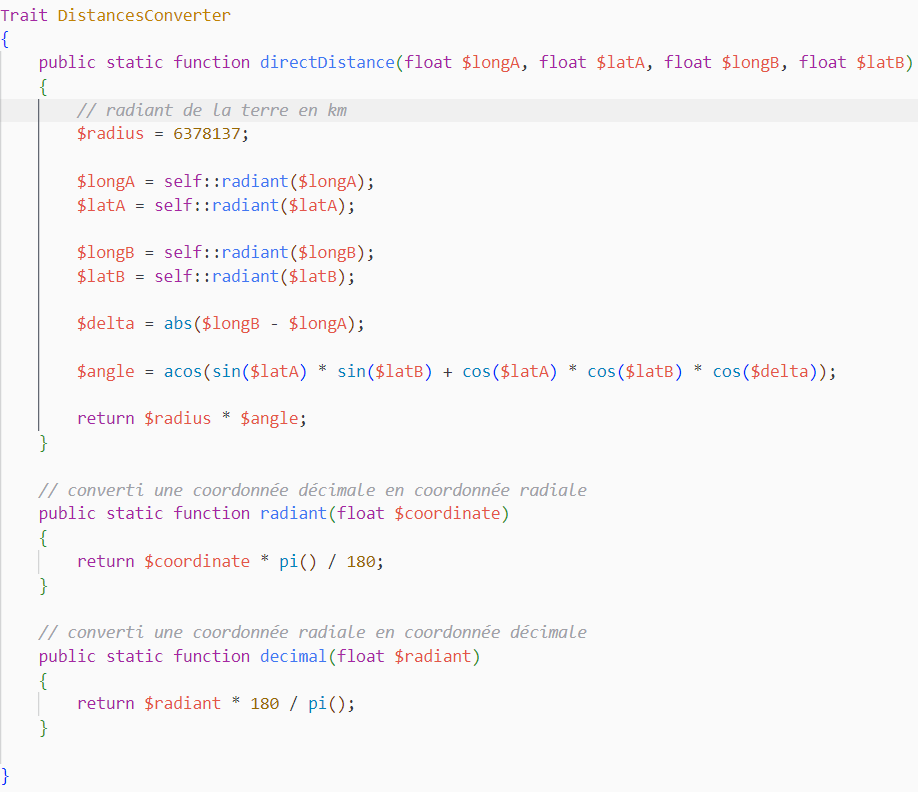
\includegraphics[width=\linewidth]{converter.png}
    \caption{Trait pour convertir des coordonnées GPS en distance}
\end{figure}

J’ai également mis en place les outils nécessaires à l’utilisation de la deuxième méthode pour l’utiliser à terme, car celle-ci permet la récupération d’informations plus riches et précises comme le temps de trajet en fonction du moyen de transport par exemple.

J’ai commencé par créer une classe avec deux méthodes distinctes pour effectuer les différentes requêtes.

\begin{figure}[!h]
    \centering
    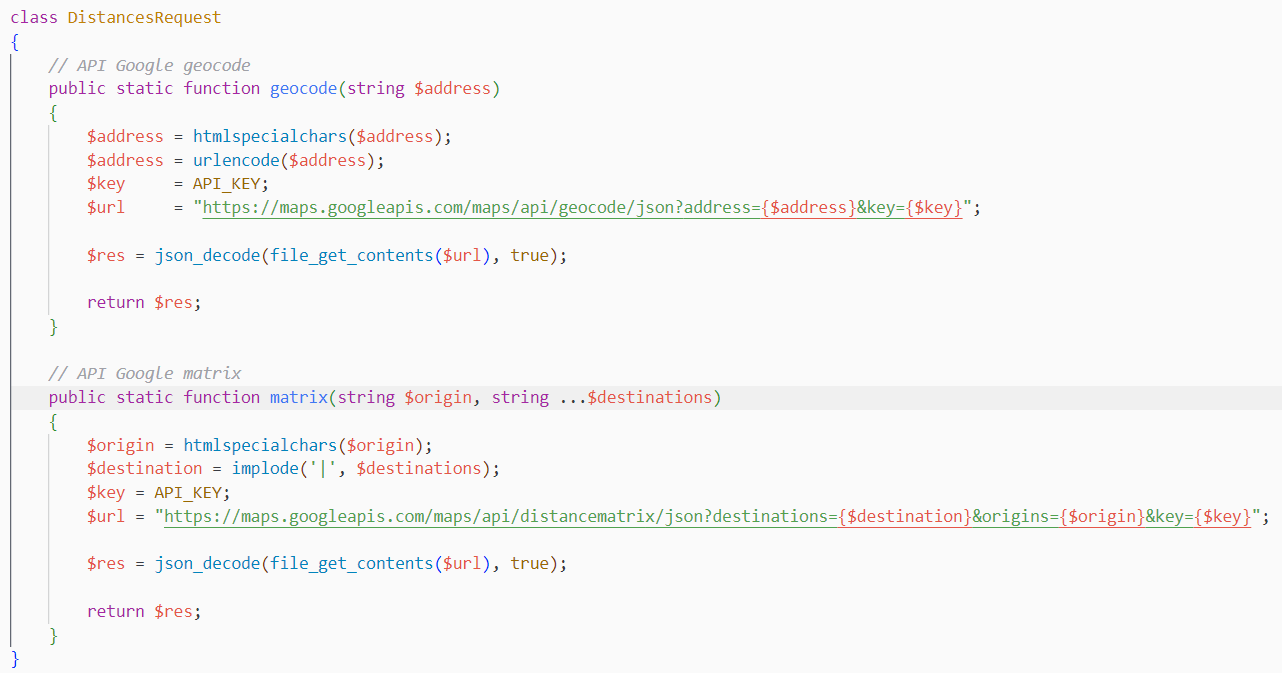
\includegraphics[width=\linewidth]{google.png}
    \caption{Composant pour envoyer des requêtes aux API Google}
\end{figure}

Les méthodes geocode et matrix récupèrent respectivement les réponses renvoyées par les API Google Geocoding et Google Matrix, sous forme de tableau associatif grâce à la fonction json\_decode pour une manipulation ultérieure.\\ \\

J’ai ensuite réalisé une classe pour la récupération et la mise en place des données géographiques dans la base de données. La récupération se base sur les méthodes de la classe \colored{DistanceRequest} , pour chaque arbitre et chaque gymnase disponibles dans la base de données (voir section sur la récupération des données).

La logique suivie par les méthodes de cette classe est d’abord de créer la colonne accueillant les coordonnées dans les tables si inexistante, puis d’insérer les coordonnées en se basant sur la réponse de l’API Google Geocoding.

À l’issu de ce processus, les tables des arbitres et des gymnases avaient toutes les deux une colonne supplémentaire avec les coordonnées géographiques de leur adresse. Ces coordonnées étaient sous format \colored{JSON} et stockaient \colored{null} si l’adresse était indisponible ou mal formatée.

\subsubsection{Matrice des distances}
\vspace{1cm}

Comme je l’ai expliqué dans l’introduction de ce chapitre, l’objectif avec ces coordonnées était de calculer la matrice des distances entre chaque adresse d’arbitre et de gymnase. 

Je me suis basé sur les outils du composant \colored{DistancesConverter} pour effectuer le calcul des distances, et j’ai ensuite stocké ces matrices sous forme de tableau associatif au format \colored{JSON} pour plus de flexibilité.

Ces matrices sont construites de façon à associer l’ID de chaque gymnase à la distance en mètres le séparant d’un arbitre, pour chaque arbitre puis de façon symétrique pour chaque gymnase.

Pour bien finir, et dans un objectif d’automatisation de ce processus dans le futur, j’ai finalement créé un composant dédié à la mise en place de ces matrices qui se base sur les classes de récupération de coordonnées et de calcul de distance à partir de celles-ci. 
Ce dernier appelle de façon procédurale les méthodes permettant de récupérer les coordonnées GPS et de calculer la matrice des distances pour chaque arbitre et chaque gymnase.
\subsection{Habilitations}
\vspace{1cm}

Un autre critère essentiel à la mise en place de l’automatisation de la désignation des arbitres était la prise en compte des habilitations des arbitres. En effet, cet algorithme devait pouvoir proposer la désignation d’arbitres habilités pour chaque match.

Le problème était que ces habilitations n’étaient pas disponibles directement dans les informations liées aux arbitres, et ne pouvaient pas être récupérées via CURL comme pour les informations précédentes. Il fallait donc pouvoir récupérer celles-ci d’une façon différente.\\

Ici encore j’ai pensé à deux méthode qui présentaient chacune leurs avantages et inconvénients :

\begin{itemize}
    \item la première méthode était de déduire ces habilitations à partir de la liste passée des désignations, en prenant en compte le type de match le plus élevé qu’avait arbitré chaque arbitre, pour en déduire un plafond d’habilitation.
    \item La deuxième méthode était de déduire les habilitations de chaque arbitre à partir du grade et du niveau de leur licence.
\end{itemize}

La première méthode présentait quelques problèmes : le plus important était le manque d’informations concernant une bonne partie des arbitres qui n’avaient pas pu arbitrer les matchs de la saison en cours. De plus, les arbitres pour lesquels les informations étaient disponibles ne reflétaient pas forcément le niveau maximum d’habilitation qu’ils possédaient. J’ai estimé un taux d’erreur avec cette méthode de l’ordre de 30\% environ.\\

Concernant la deuxième méthode, il faut savoir que les habilitations d’arbitres ne sont pas toujours définies par leur niveau et grade de licence, mais que ces données sont quand même fortement liées aux habilitations. Le taux d’erreur avec cette méthode était de l’ordre de 15\%.\\

Le taux d’erreur étant plus faible, j’ai donc décidé de me reposer sur la deuxième méthode pour effectuer la déduction des habilitations, et de mettre en place une interface graphique permettant la mise à jour de celles-ci.  Cette interface permettrait aux gestionnaires d’effectuer les modifications nécessaires pour les arbitres pour lesquels les habilitations ne correspondraient pas.

Pour effectuer la mise en place des habilitations initiales des arbitres, j’ai créé une unique méthode dans une classe dédiée à cette tâche

\newpage

\begin{figure}[!h]
    \centering
    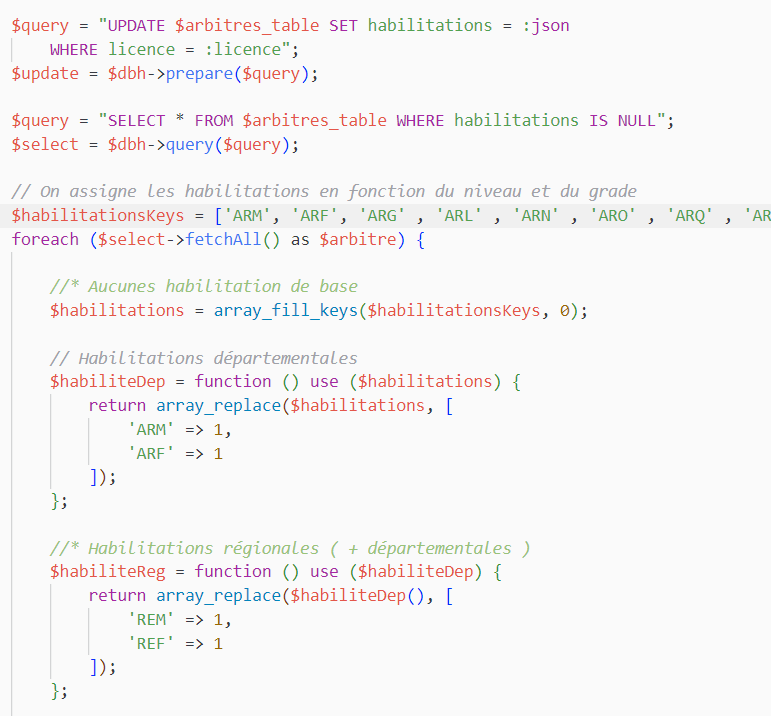
\includegraphics[width=10cm]{habilitations_code.png}
    \caption{Mise en place des requêtes et fonction nécessaire à la mise en place des habilitations}
\end{figure}

\begin{figure}[!h]
    \centering
    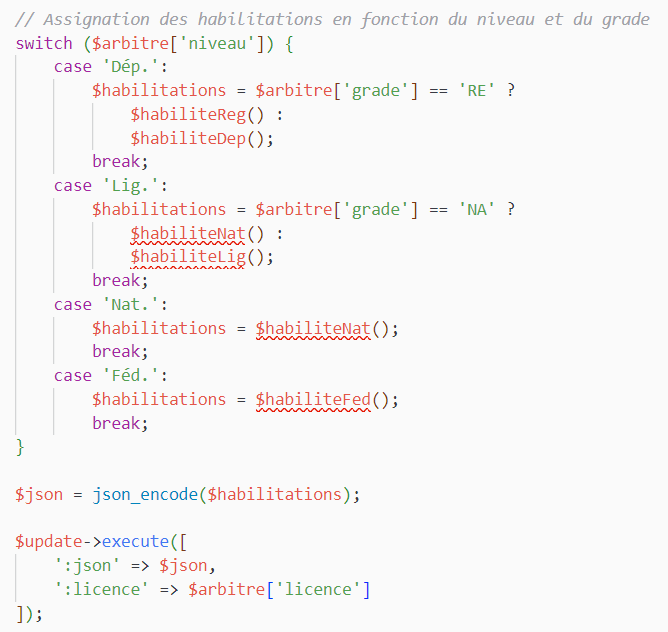
\includegraphics[width=10cm]{habilitations_code2.png}
    \caption{Détermination des habilitations initiales de l'arbitre}
\end{figure}

\newpage 

Les différents types d’habilitations nous ont été indiqués par notre tuteur et sont définis par des critères subjectifs basés sur les différents types de matchs possibles. Les clés correspondantes à ces habilitations sont stockées dans un tableau indexé, et initialisées à zéro pour chaque arbitre. Cette valeur signifie que les arbitres n’ont aucunes habilitations au départ.  

Puis en fonction du niveau et du grade de leur licence, les habilitations des arbitres sont modifiées à un pour chaque clé correspondante au niveau d’habilitation associé. Ces habilitations étant cumulées de façon croissante à chaque niveau supplémentaire, j’ai utilisé la fonction \colored{array\_replace()} pour retourner un tableau des habilitations complètes de chaque arbitre.

Une fois ce tableau défini, il fallait finalement l’insérer sous format \colored{JSON} dans la base de données. Pour faire cela, j’ai utilisé la méthode \colored{json\_encode()} sur le tableau des habilitations et je l’ai inséré à l’aide d’une requête SQL de type INSERT. \\ \\ 

Une fois les habilitations initiales insérées dans la base de données, j’ai ensuite pu travailler sur l’interface de mise à jour de celles-ci. 
J’ai donc mis en place une page annexe qui affiche la liste de tous les arbitres, auxquels on associe la liste de toutes les habilitations préremplies sous forme de SELECT. Chaque select permet de choisir entre “Oui/Non”, permettant ainsi de choisir ou non d’accorder l’habilitation à l’arbitre voulu. 

\begin{figure}[!h]
    \centering
    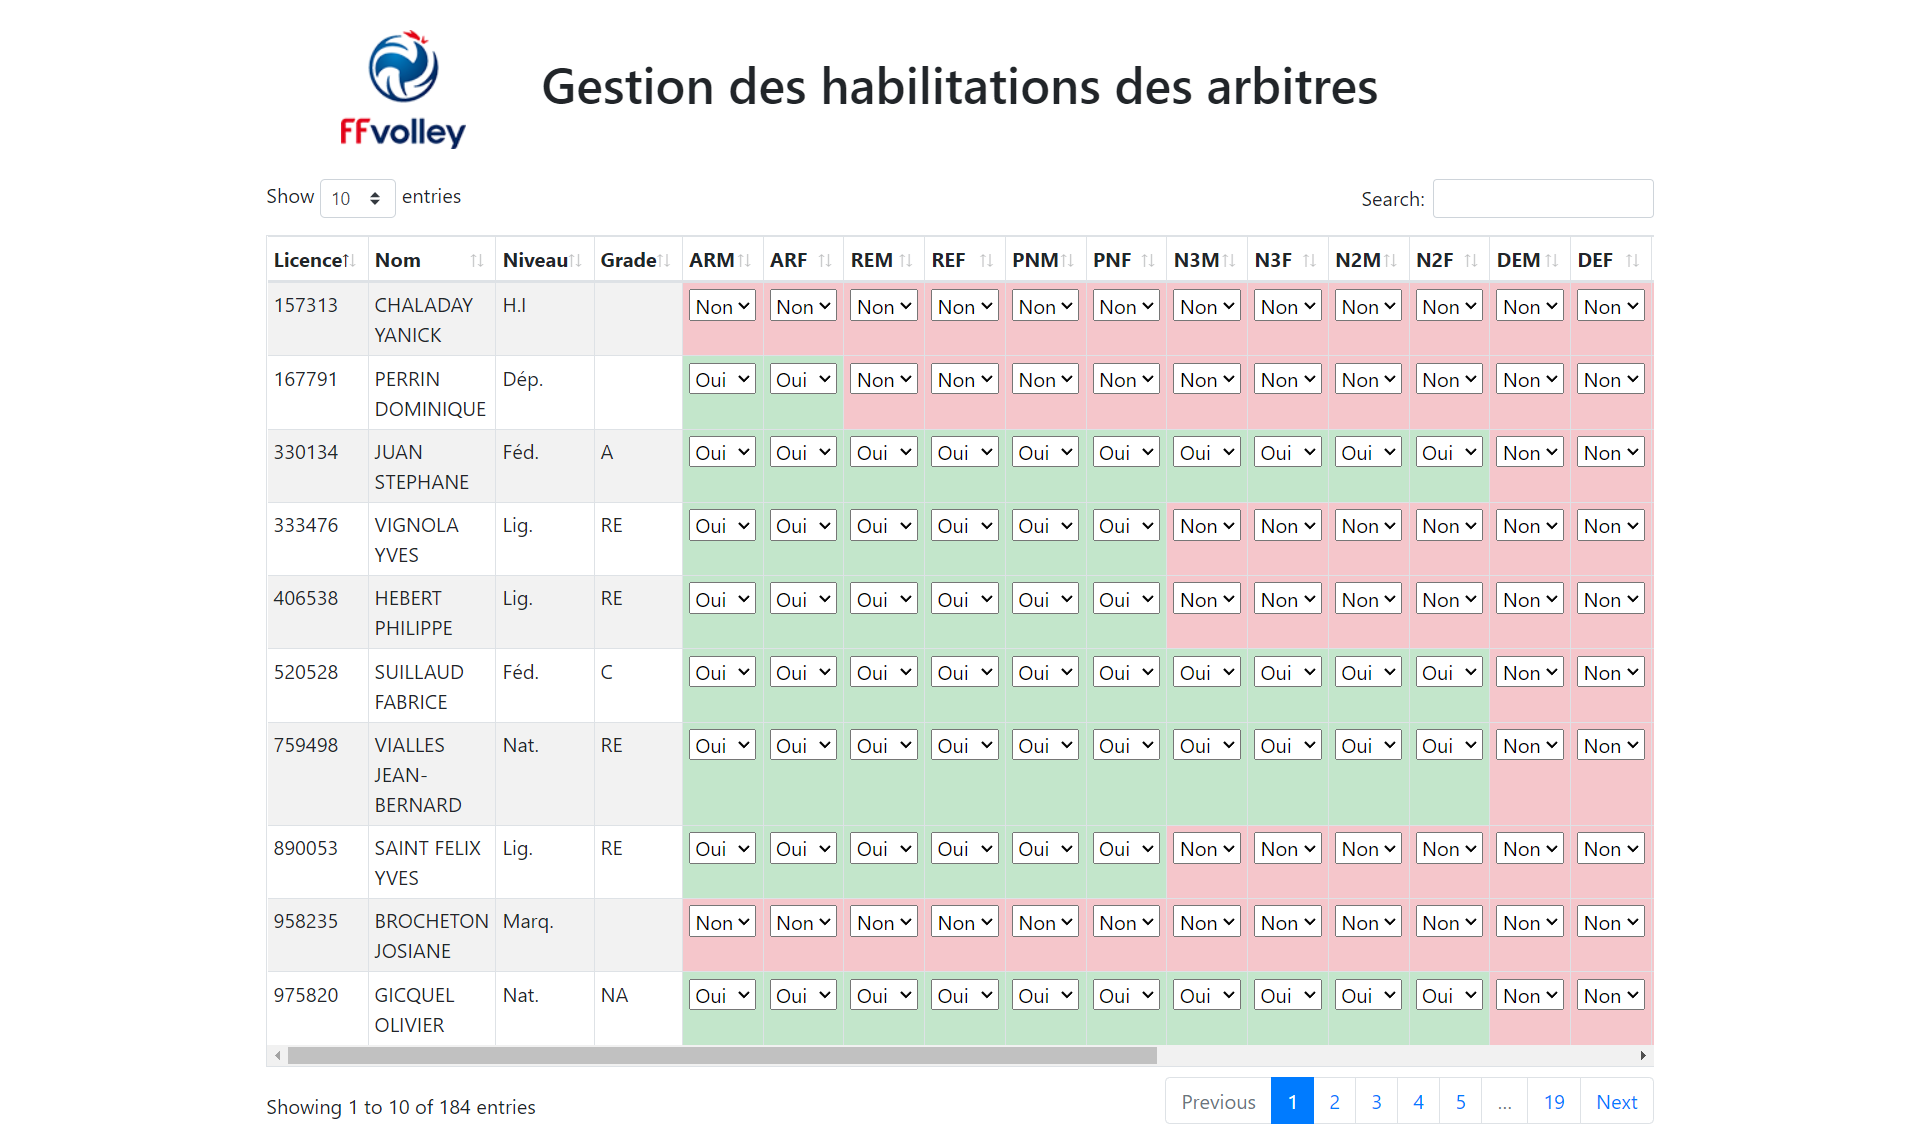
\includegraphics[width=\linewidth]{habilitations.png}
    \caption{Interface de mise à jour des habilitations}
\end{figure}

\newpage

Un script javascript permet ensuite au changement d’un select, d’envoyer via ajax le numéro de licence et les nouvelles informations d’habilitations à une page dédiée de notre back-end. Cette page récupère ensuite les habilitations actuelles de l’arbitre, les transforme en tableau associatif grâce à la fonction \colored{json\_decode()}, puis met à jour l’habilitation voulue. Elle encode ensuite ce nouveau tableau sous format JSON et l’insère dans la base de données.

Pour plus de détails concernant la partie graphique de cette page, merci de vous reporter au chapitre sur les interfaces.
\subsection{Mise à jour}
\vspace{1cm}

Toutes les informations récupérées et calculées jusqu’à maintenant, devaient pouvoir être mises à jour régulièrement via un script simple. J’ai donc mis en place un composant spécialement dédiée à cette action, qui lance de façon procédurale la mise en place de la base de données et la récupération complète de tous les éléments précédemment introduits.

Cette classe prend en paramètre des identifiants fédéraux valides, nécessaires au lancement des méthodes CURL, ainsi qu’une clé API Google active.

\begin{figure}[!h]
    \centering
    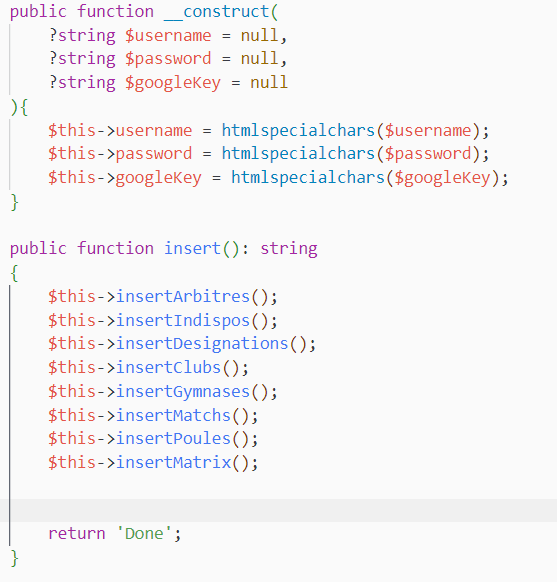
\includegraphics{update_code.png}
    \caption{Méthode principale du composant de mise à jour de la BDD}
\end{figure}

Un appel à la méthode \colored{insert()} de cette classe crée la base de données définie dans le fichier de configuration \colored{globals.php} (voir configuration), en prenant en compte le nom des tables et colonnes définies dans le fichier \colored{config.json}, puis insère toutes les données nécessaires au projet depuis les différentes classes de celui-ci.

\section{Algorithme}
\vspace{1cm}

Une fois tous les outils en main, j’ai pu travailler sur l’algorithme d’automatisation des désignations. Pour rappel, cet algorithme devait prendre en compte trois critères importants : les disponibilités des arbitres, leurs habilitations et la distance qui les sépare du lieu de la rencontre.

L’étape la plus importante a été de réfléchir à une façon de procéder aux désignations selon ces critères et de proposer celles-ci sans les valider directement.

Dans un souci de maintenabilité et d’évolutivité, j’ai fractionné cet algorithme en plusieurs composants qui font chacun référence à une étape ou sous-étape de celui-ci. De cette façon, la compréhension de l’algorithme devenait plus facile et son amélioration plus accessible.

\subsection{Principe général}
\vspace{1cm}

Une première étape a été de regrouper tous les matchs de la période voulue par date, puis de vérifier les disponibilités des arbitres pour chacun d’entre elles et d’obtenir un tableau des arbitres disponibles du jour.\\

Il fallait ensuite prendre en compte individuellement pour chaque match les habilitations de ces arbitres, pour en tirer une sous liste d’arbitres potentiels.

À partir de cette sous-liste d’arbitres potentiels pour chaque match, il fallait ensuite prendre en compte le critère des distances de façon assez subtile pour ne pas influer complètement sur les désignations.

\begin{figure}[!h]
    \centering
    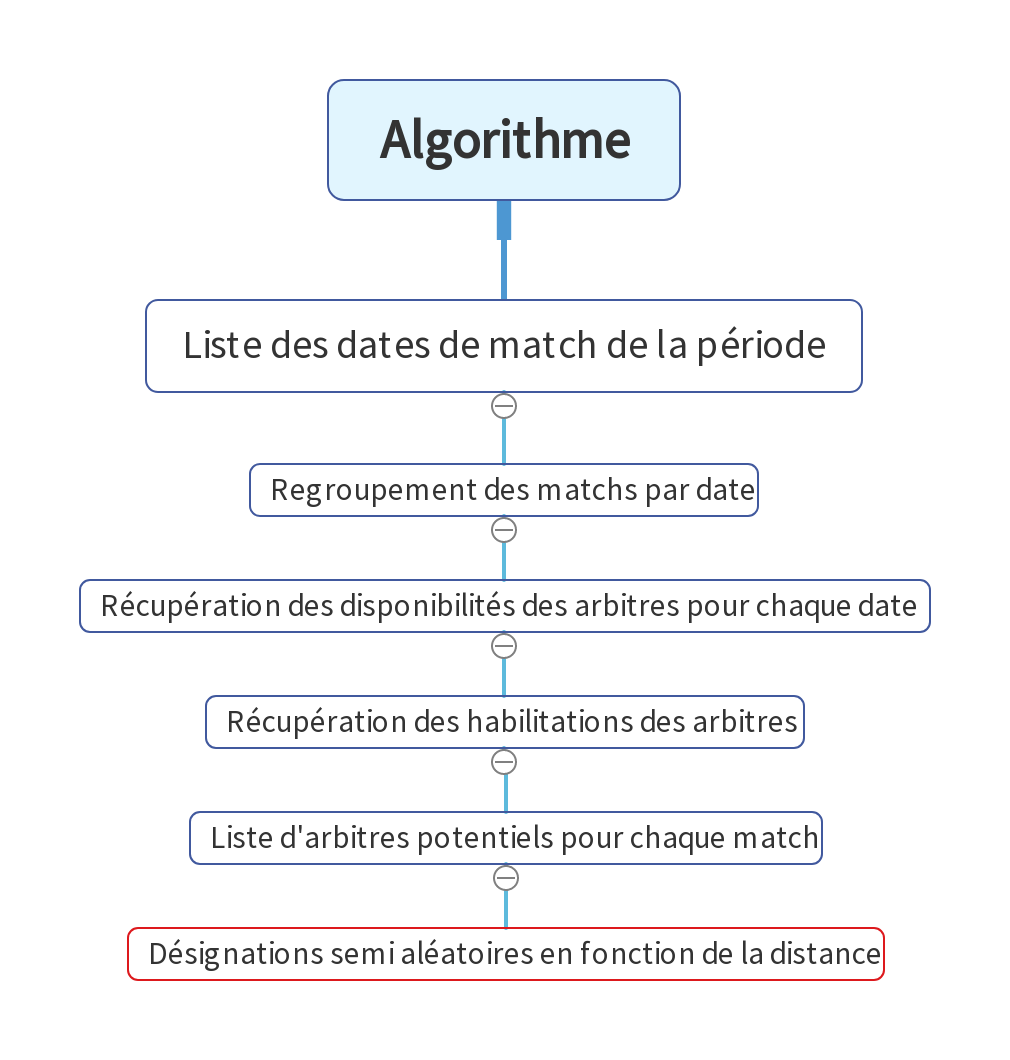
\includegraphics[height=15cm]{algorithme.png}
    \caption{Logique suivie par l'algorithme}
\end{figure}


\subsection{Etape 1 : regroupement des matchs par date}
\vspace{1cm}

Le regroupement des matchs par date était une première étape importante car elle devait également permettre de trier les matchs par type pour la suite de l’algorithme. 

En effet, les matchs peuvent être de type tournois dans le cas ou plusieurs d’entre eux se déroulent au même endroit, ou de type uniques dans le cas contraire. 
Ainsi, en faisant ce tri à ce moment, il était possible de prendre en compte différemment les désignations dans la suite du programme.

De plus, l’algorithme devait pouvoir effectuer les désignations d’une période donnée, ou de l’ensemble des matchs de la saison si aucune date n’était fournie. Il fallait donc également prendre en compte ces deux scénarios différents.

Le composant qui s’occupe de cette première étape prend donc en paramètres les dates de la période souhaitée, qui ont comme valeur par défaut les dates de la période allant d’aujourd’hui à la fin de saison.

\vspace{1cm}

\begin{figure}[!h]
    \centering
    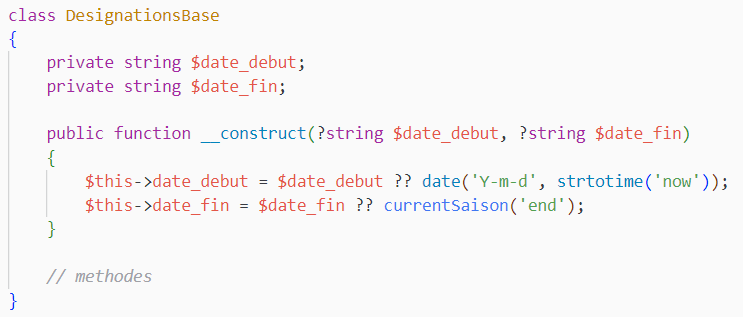
\includegraphics[width=0.75\linewidth]{designations1}
    \caption{Constructeur du composant principal}
\end{figure}

\vspace{1cm}

Ce composant sous forme de classe possède la méthode \colored{group()} qui permet de regrouper les matchs de la période par date, tout en faisant le tri entre les matchs tournois et uniques. 
Cette méthode récupère la liste des dates distinctes de cette période puis associe, pour chaque date, la liste des matchs tournois et uniques à leur tableau des matchs respectifs.

\newpage 

\begin{figure}[!h]
    \centering
    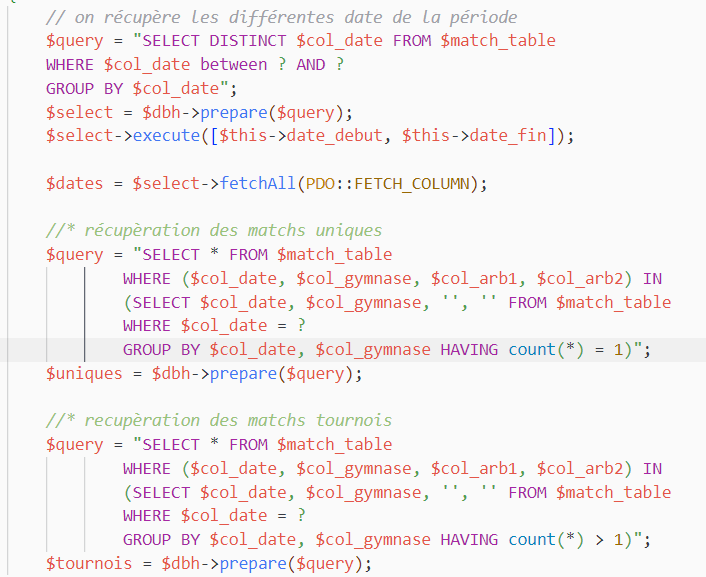
\includegraphics[width=0.75\linewidth]{group1}
    \caption{Préparation des requêtes qui permettent de grouper les matchs}
\end{figure}

\subsection{Etape 2 : récupération des arbitres potentiels}
\vspace{1cm}

Cette liste de dates associées à leurs matchs m’a ensuite permis d’appliquer le premier critère de disponibilité. Pour vérifier les disponibilités des arbitres de chaque match, j’ai réutilisé des méthodes implémentées lors de l’insertion des indisponibilités et des désignations dans la base de données. Alliées ensemble, ces méthode permettent de définir si un arbitre est disponible pour une date donnée. 
Elles m’ont donc permis d’attacher à chaque match un tableau des arbitres disponibles.\\

Ensuite, il a fallut définir pour chaque match une sous liste d’arbitres potentiels habilités à partir de ces tableaux d’arbitres disponibles. 
Pour faire cela j’ai utilisé la classe dédiée au filtre des habilitations en appliquant pour chaque arbitre potentiels une méthode qui renvoi un booléen si l’arbitre est habilité ou non pour le match voulu.
\subsection{Etape 3 : processus de sélection}
\vspace{1cm}

J’avais donc pour chaque match une liste d’arbitres habilités potentiels. La prochaine étape était donc de procéder aux désignations. \\

Contrairement aux matchs uniques, les matchs tournois doivent avoir un arbitre pour chaque groupe de trois matchs de la même poule. Il fallait donc prendre en compte différemment la sélection en fonction du type de match.

Autre contrainte mineure, il fallait que la désignation prenne en compte le nombre exacte d’arbitres pour chaque match.

\subsubsection{Matchs uniques}
\vspace{1cm}

La seule chose à prendre en compte pour la sélection des arbitres pour les matchs uniques était le nombre d’arbitres nécessaires pour chaque match. Cette donnée n’est pas explicite et dépend de la poule et du niveau du match. 
J’ai donc créé une méthode dans la classe \colored{DesignationsBase} qui permet de déterminer si un match demande deux arbitres ou non.

\begin{figure}[!h]
    \centering
    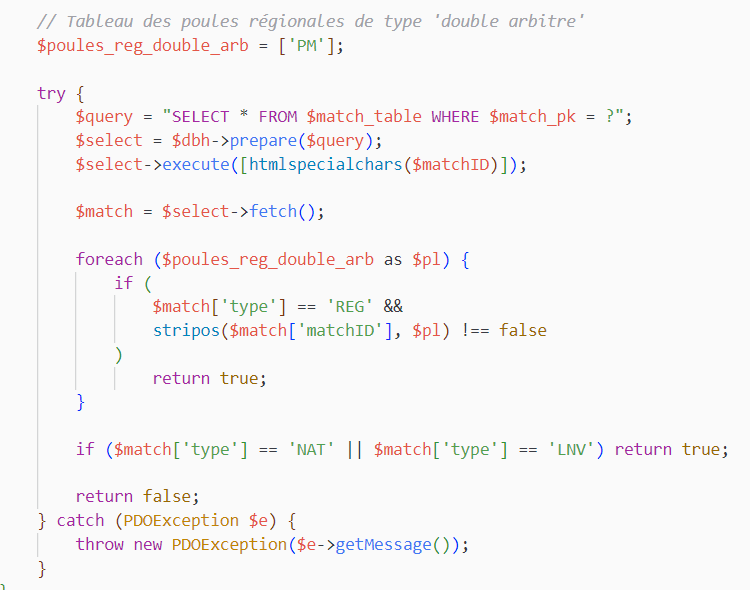
\includegraphics[width=0.75\linewidth]{double}
    \caption{Détermination du nombre d'arbitres pour le match}
\end{figure}

Le nombre d’arbitres est déterminé en fonction du niveau du match (régional ou national), et prend en compte les exceptions. \\

Une fois le nombre d’arbitres défini, la distance entre chaque arbitre potentiel est récupérée dans la base de données et associée avec les arbitres dans un tableau trié par distance croissante. Ce tableau final permet de procéder aux désignations de façon semi aléatoire en augmentant progressivement la probabilité de sélection des arbitres en fonction de leur distance avec le gymnase.

\begin{commentaire}
Un score aléatoire est attribué à chaque arbitre. Ce nombre aléatoire est compris entre 0 et 100, puis multiplié par une valeur allant de 2 à 0,5. Les arbitres voient leur score ajusté à la baisse entre ces deux valeurs en fonction de leur distance avec le gymnase.
Ceci induit alors que le score de l’arbitre le plus proche est multiplié par deux et celui du plus éloigné est divisé par deux.
\end{commentaire}

De cette façon, les arbitres dont la distance avec le gymnase est faible ont plus de chance d’être sélectionnés par l’algorithme, sans pour autant enlever complètement la probabilité de sélection des arbitres dont la distance est plus élevée.

Une fois un arbitre sélectionné, celui-ci est ensuite retiré du tableau global des arbitres disponibles du jour pour ne plus être resélectionné pour d’autres matchs le même jour.

\subsubsection{Matchs tournois}
\vspace{1cm}

Le processus de sélection des matchs tournois se rapproche de celui des matchs uniques.
La sélection reste semi aléatoire de façon à mettre l’accent sur les arbitres dont la distance avec le gymnase est plus faible.  \\

Cependant, par souci d’optimisation, il fallait pouvoir désigner un seul arbitre par paquet de trois matchs de la même poule d’un tournois. 
De cette façon, un arbitre se déplacerait pour arbitrer trois match consécutifs d’un tournois.

J’ai pris en compte cette différence en ajoutant quelques ligne de code permettant de désigner le même arbitre pour trois match consécutif de la même poule.
\subsection{Validation}
\vspace{1cm}

Une particularité de ces désignations automatiques était de les rendre temporaires jusqu’à validation par un gestionnaire fédéral. Cette étape de validation devait alors se faire en deux temps : une étape pour procéder aux désignations temporaires, puis une étape de validation de ces dernières.\\

Pour faire face à ce problème, j’ai pensé à mettre en place une table temporaire identique à celles des matchs, qui permettrait d’afficher les désignations d’arbitres temporaires tout en permettant ensuite leur validation dans la table officielle.\\

En effet, notre page principale des désignations est basée sur la table des matchs, et la création d’une table identique permet alors de faciliter l’affichage des nouvelles désignations sans devoir reconfigurer les désignations manuelles.

La validation des désignations automatiques se fait donc en basculant alors les informations de cette table temporaire vers la table officielle des matchs.
\subsection{Rapport}
\vspace{1cm}

Une demande postérieure concernant cet algorithme a été de pouvoir suivre le procédé de désignation des arbitres avec un rapport complet des étapes. 
Grâce à la découpe des différentes fonctions de celui-ci, l’ajout de ce rapport a été rapide en ajoutant simplement l’écriture de descriptions durant chaque étape du processus.

\begin{figure}[!h]
    \centering
    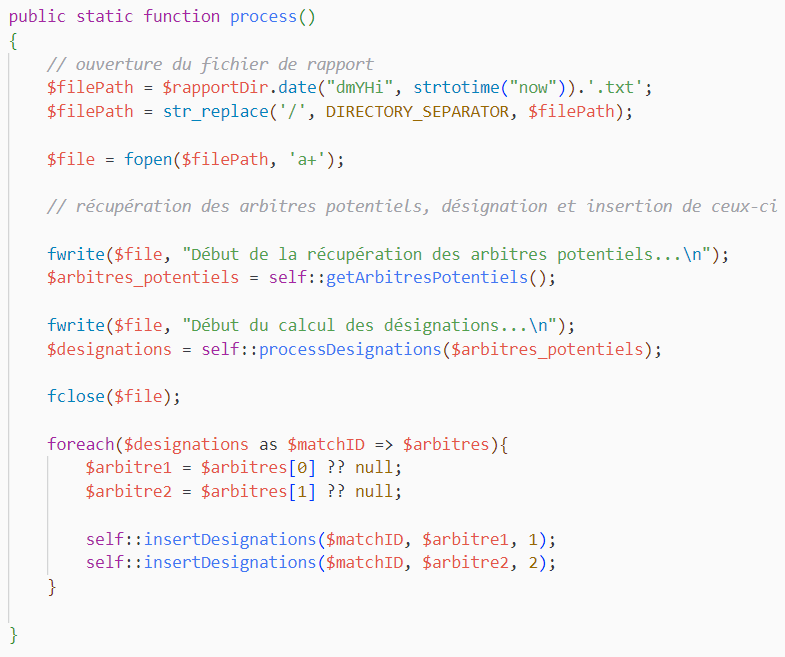
\includegraphics[width=0.75\linewidth]{process}
    \caption{Methode appellée pour lancer l'algorithme - incorporation du rapport d'erreurs}
\end{figure}


\section{Interface}
\vspace{1cm}


Le dernier axe important de la transition numérique qui m’a été confiée, a été la refonte de l’interface de gestion des arbitres et y intégrant les nouveaux outils créés. Il m’a fallu moderniser cette interface en gardant la nouvelle identité du site mise en place par mon tuteur.

Au total, l’interface devait posséder trois pages distinctes pour chacune des fonctionnalités principales de cette partie du site. Celles-ci sont :

\begin{itemize}
    \item L’interface principale pour les désignations des arbitres
    \item Une interface secondaire pour la gestion des habilitations.
    \item Une dernière interface pour la gestion des poules à afficher ou non
\end{itemize}

\vspace{1cm}

\begin{figure}[!h]
    \centering
    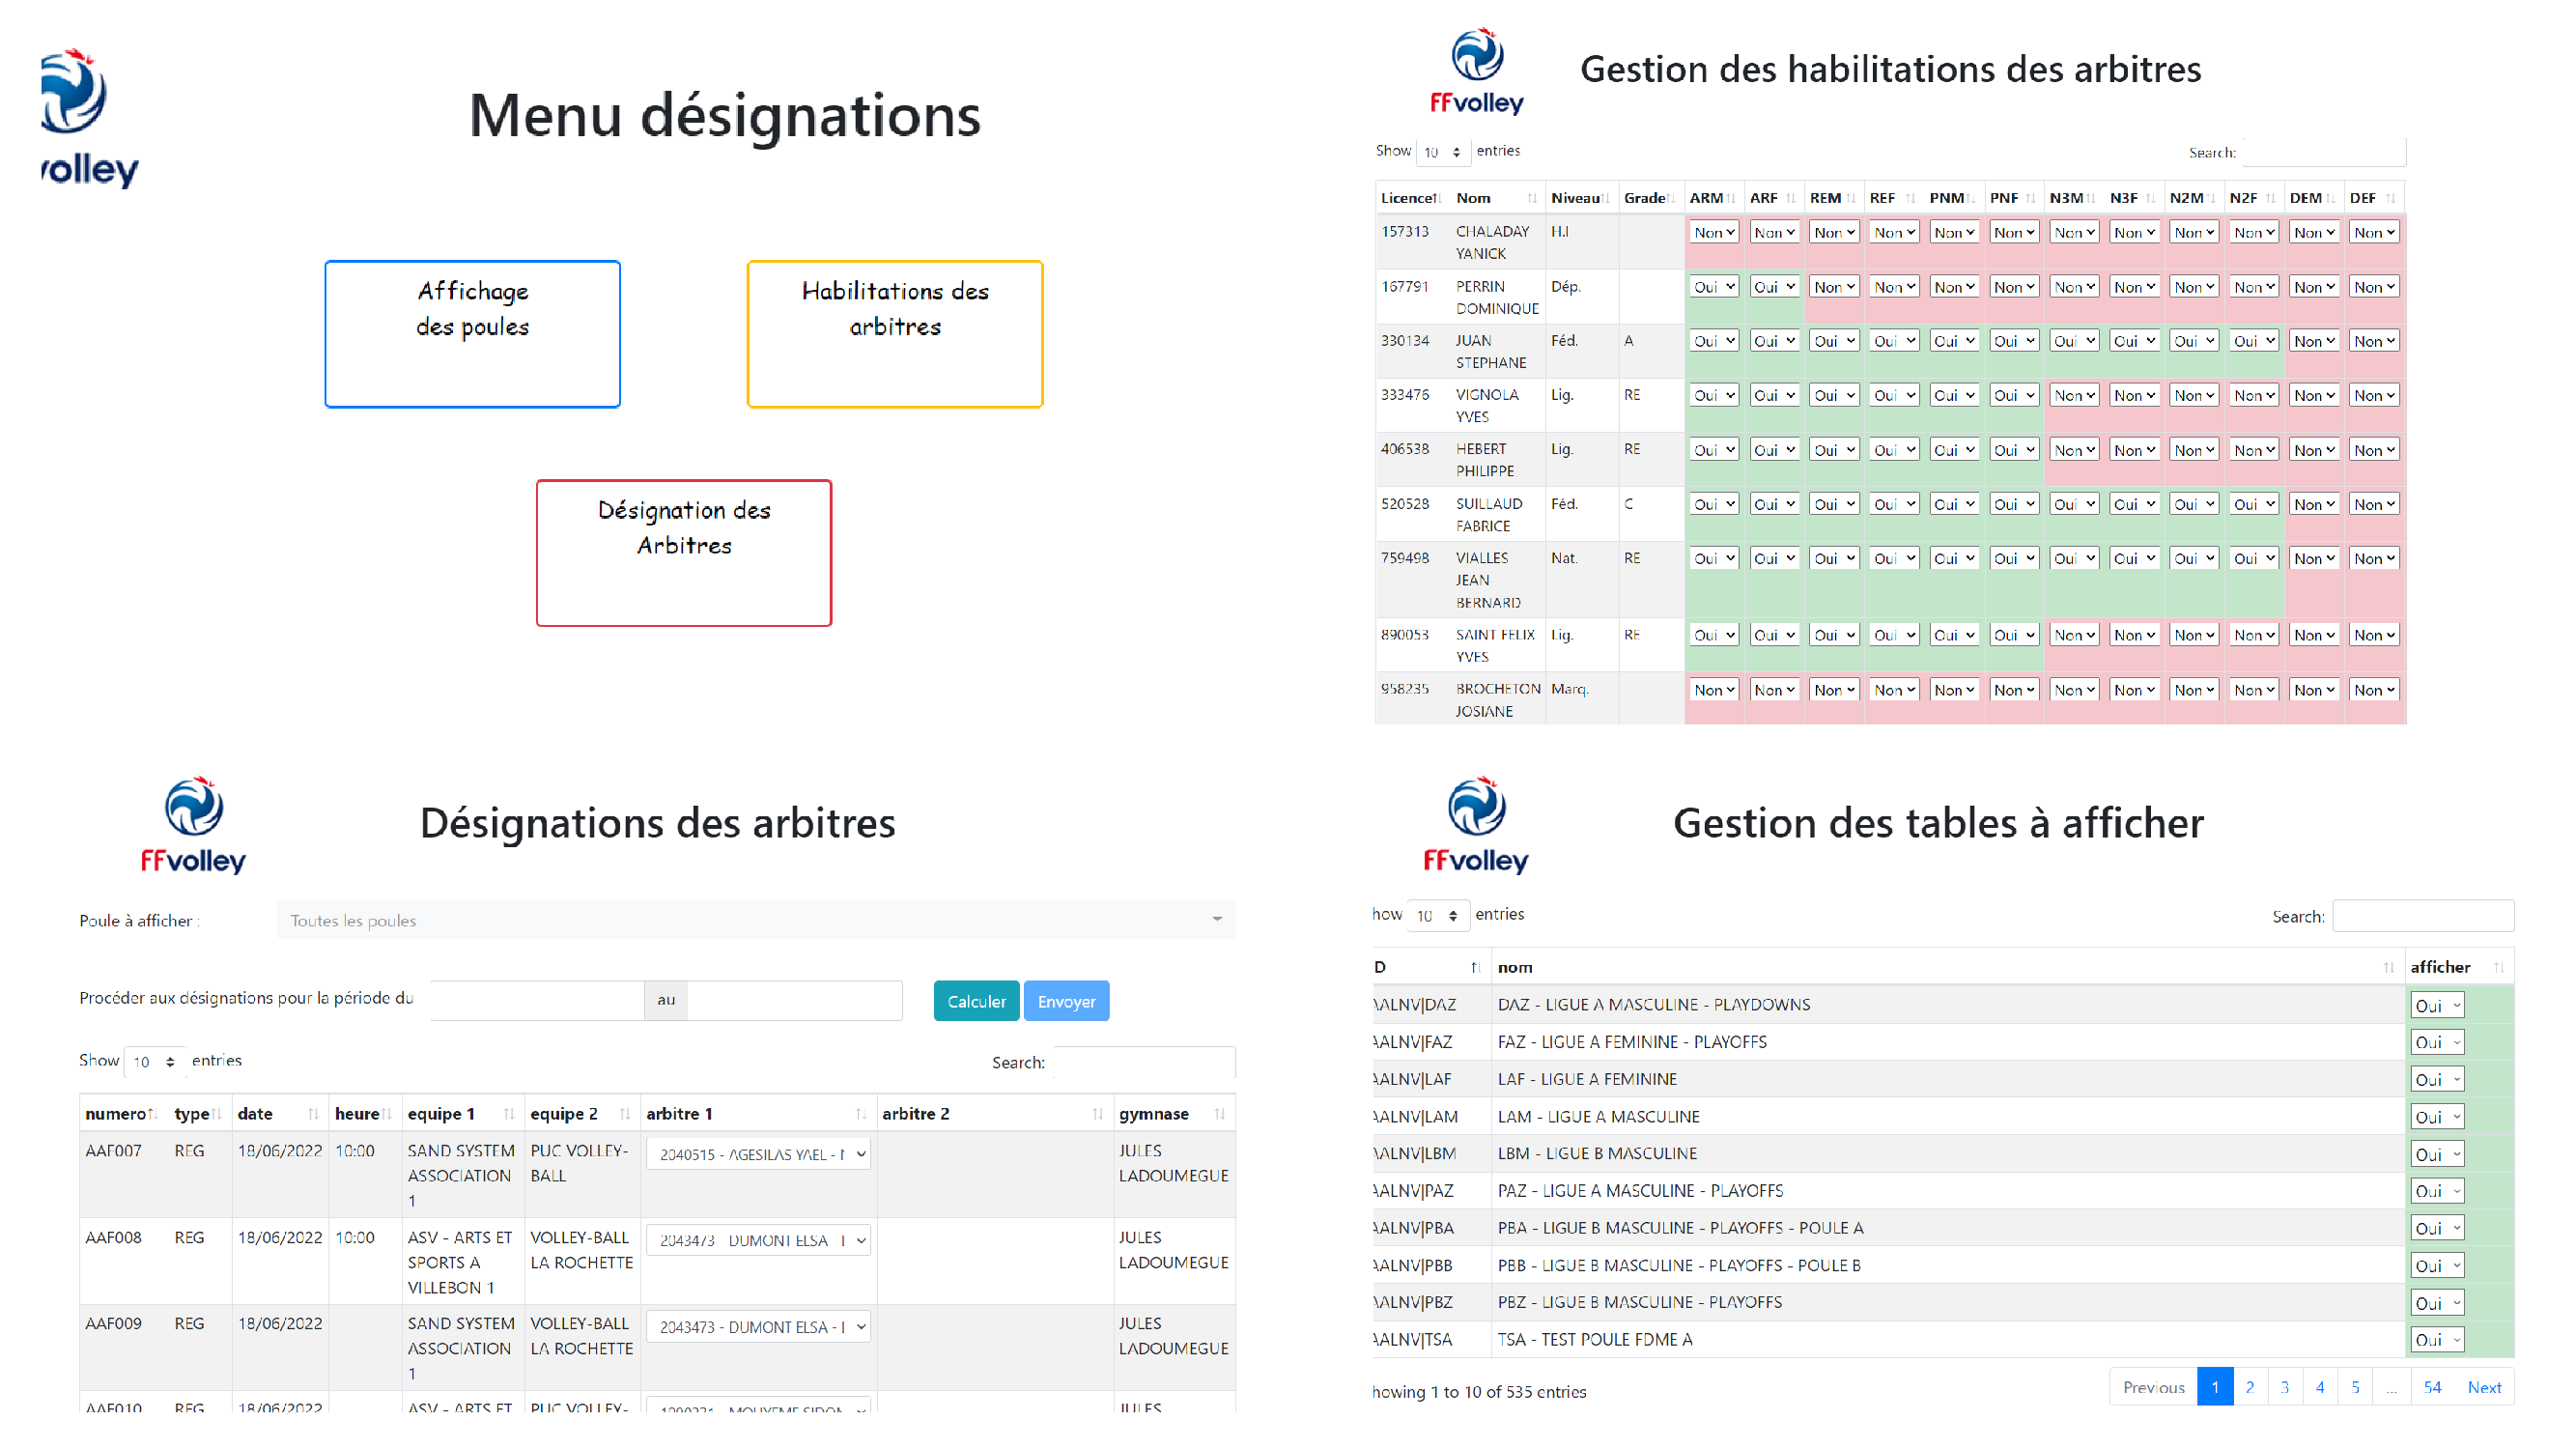
\includegraphics[width=\linewidth]{pages}
    \caption{Les différentes pages de l'interface}
\end{figure}

\vspace{1cm}

Ces interfaces exclusivement composées de tableaux. Ceux-ci devaient faciliter l’expérience utilisateur en intégrant une pagination, un tri par colonne et une barre de recherche.

Heureusement, l’outil \colored{Datatables}  permettait de répondre à l’ensemble de ces contraintes. 
Cet outil basé sur JQuery permet d’intégrer plusieurs fonctionnalités à un tableau html dont la pagination, la barre de recherche et le tri en fonction des colonnes.\\ \\

Pour la réalisation de ces pages, j’ai d’abord procédé au maquettage de l’application avec le logiciel dédié Adobe XD. Le but était de mettre en place un schéma visuel à suivre qui me permettrait de me concentrer uniquement sur l’implémentation du côté technique.

Une fois cette maquette réalisée et validée par mon tuteur, je me suis donc basé sur cette celle-ci pour réaliser mes pages.\\

Pour faciliter le côté responsive, et pour être en accord avec les outils déjà utilisés pour ce projet, j’ai utilisé la librairie Bootstrap pour le côté statique et JQuery pour le côté dynamique. \\

Faisant partie d’un intranet fermé au public, le référencement de ces pages n’était pas une priorité. J’ai cependant tout de même structuré ces pages en exploitant au mieux les balises html de chaque élément composant celles-ci, afin d'exploiter au moins le référencement naturel.
\subsection{Liste des matchs}
\vspace{1cm}

L’interface principale devait intégrer la liste des matchs complets à venir pour le reste de la saison. Elle devait également permettre le tri de ces matchs en fonction des différentes poules possibles sans recharger la page.\\

J’ai mis en place un composant sous forme de classe permettant de gérer ces deux différents scénarios, et de renvoyer au choix le tableau de tous les matchs à venir ou le tableau des matchs à venir d’une poule.
Pour fonctionner, cette classe prend en paramètre l’ID d’une poule et renvoi alors le tableau html composé de tous les matchs à venir associés, récupérés depuis la base de données. 
Ce paramètre peut être nul et renvoi dans ce cas la liste complète des matchs à venir sans distinction de poules.

\begin{figure}[!h]
    \centering
    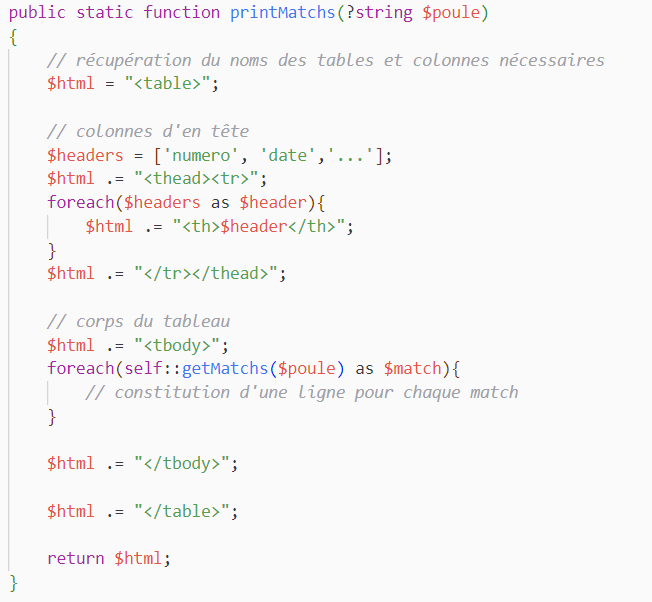
\includegraphics{table}
    \caption{Méthode de construction de tableau pour une poule}
\end{figure}

\newpage

De cette façon, je n’avais qu’à attacher un évènement au changement du SELECT affichant les poules, qui enverrait via AJAX la valeur de celle-ci à une page annexe. Cette page n’aurait alors qu’à renvoyer le bon tableau grâce à cette méthode.

\begin{commentaire}
AJAX (Asynchronous Javascript and XML) est une méthode permettant de faire des requêtes à un serveur web de façon asynchrone, et de récupérer la réponse de celui-ci sans recharger la page.
\end{commentaire}

Pour faciliter l’envoi et la gestion de ces requêtes, j’ai utilisé la bibliothèque JQuery déjà très largement utilisée dans le cadre de cette transition numérique.

\begin{figure}[!h]
    \centering
    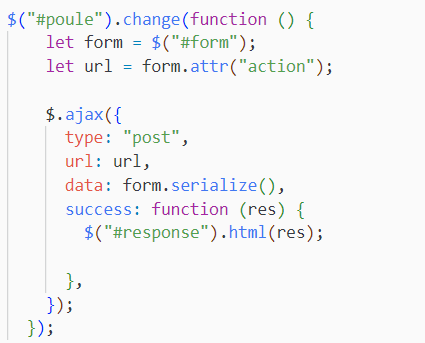
\includegraphics{ajax}
    \caption{Fonction AJAX au changement d'une poule}
\end{figure}


\subsection{Désignations}
\vspace{1cm}

L’interface actuelle du site de la fédération rend la désignation des arbitres chronophage car celle-ci demande d’effectuer plusieurs clicks afin de désigner les arbitres d’un match.

\begin{figure}[!h]
    \centering
    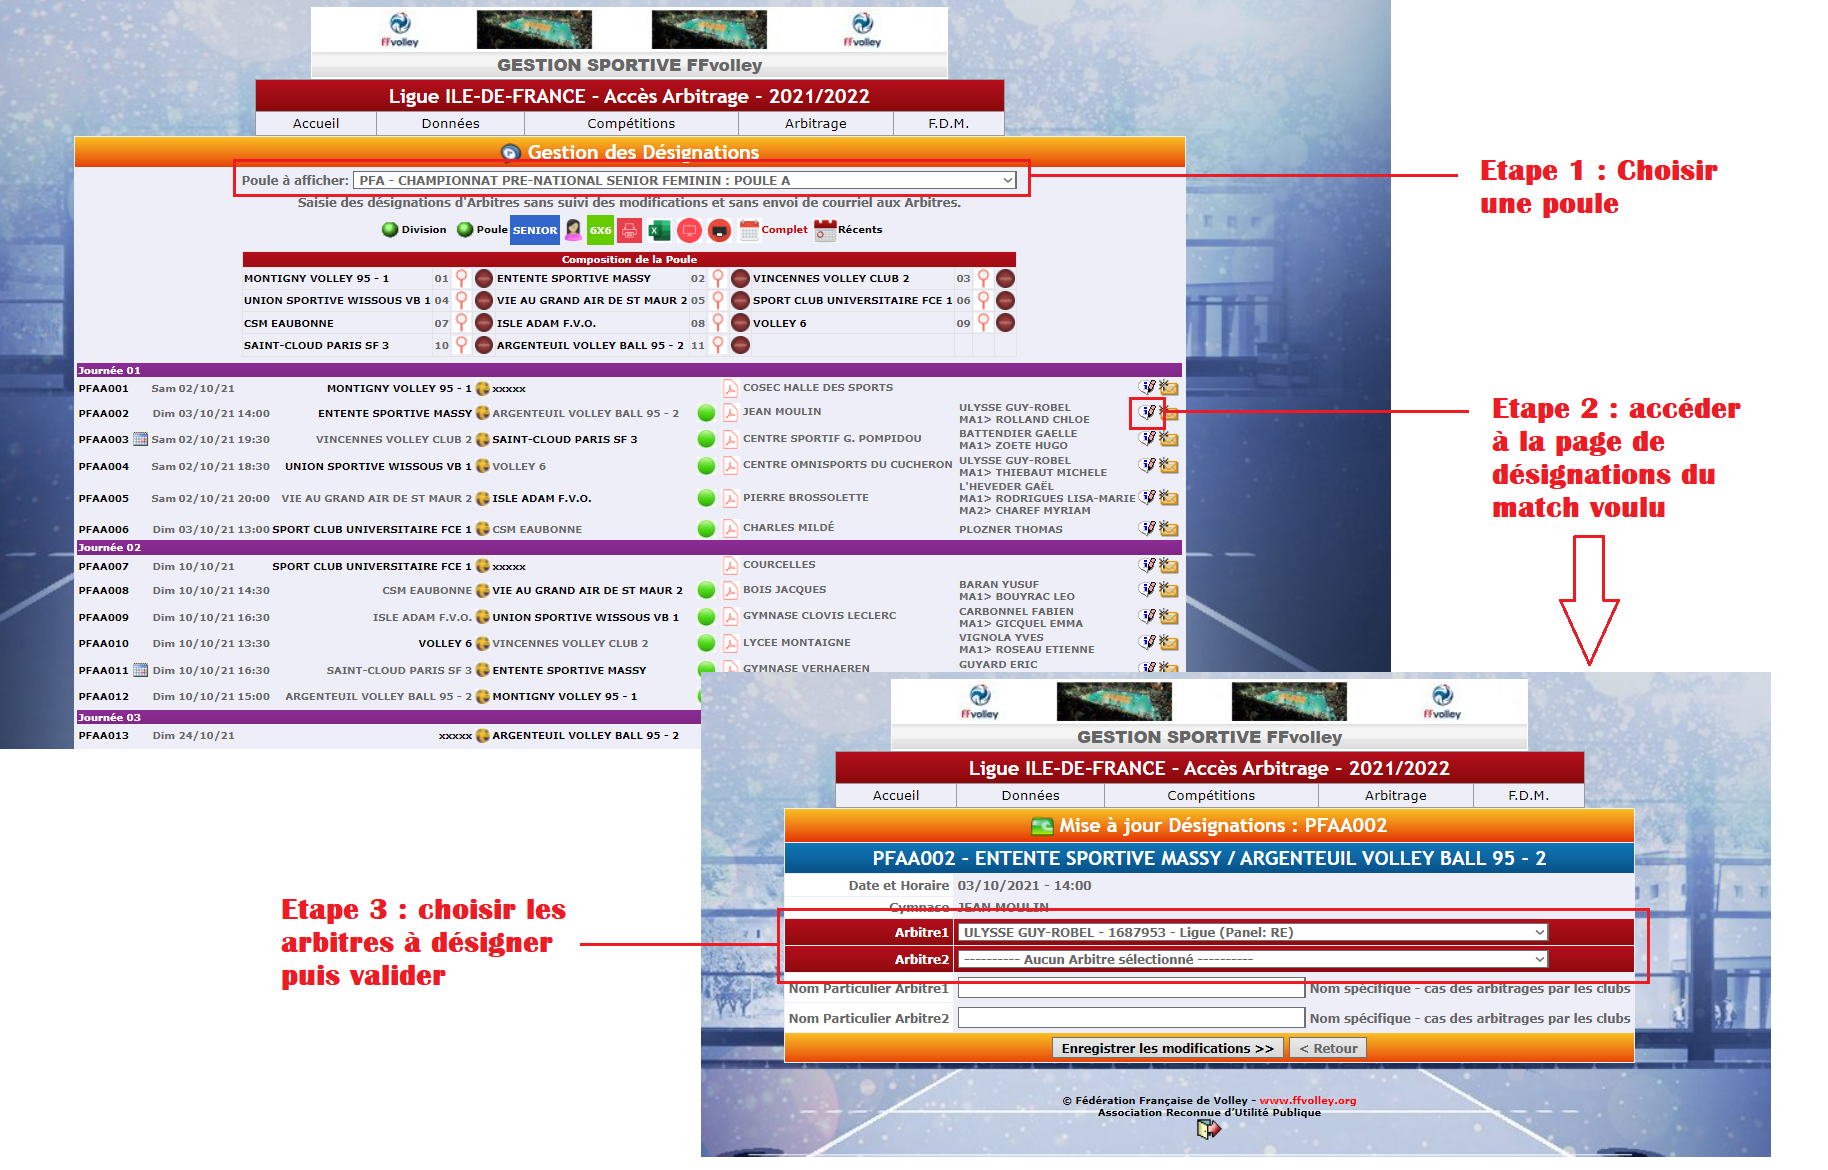
\includegraphics[width=\linewidth]{designation_avant}
    \caption{Processus de désignation des arbitres actuel}
\end{figure}

La nouvelle interface devait également servir à lancer l’algorithme d’automatisation des désignations, mais également permettre de procéder aux désignations manuellement tout en offrant le maximum d’informations possibles concernant les arbitres à désigner, le tout sur la même page. \\

Les désignations manuelles devaient pouvoir se valider de façon dynamique via AJAX, tandis que celles proposées par l’algorithme devaient pouvoir être validées via un bouton.

\begin{figure}[!h]
    \centering
    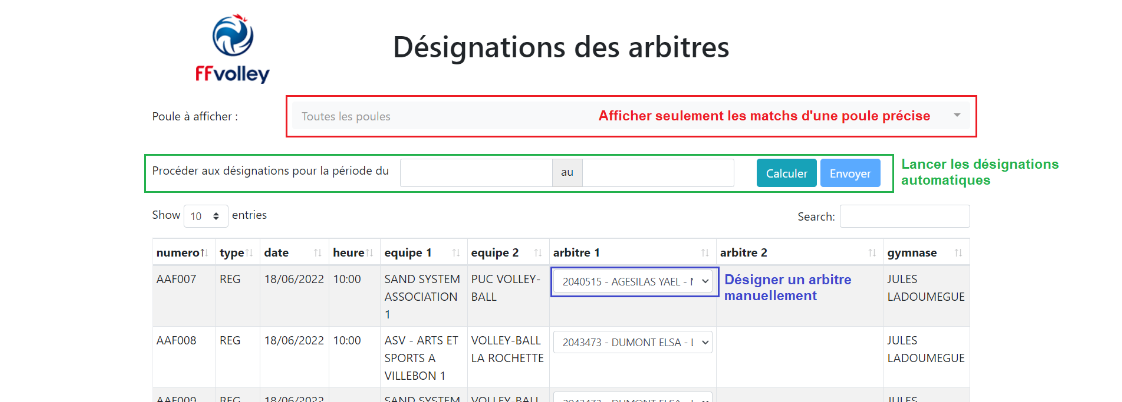
\includegraphics[width=\linewidth]{designations_mtn}
    \caption{Centralisation des informations sur la nouvelle interface}
\end{figure}

\newpage

\subsubsection{Récupération des arbitres}
\vspace{1cm}

Le calcul des disponibilités des arbitres pour chaque match étant trop long à effectuer au chargement de la page, celles-ci sont récupérées via AJAX quand l’utilisateur clique sur un SELECT.

\begin{figure}[!h]
    \centering
    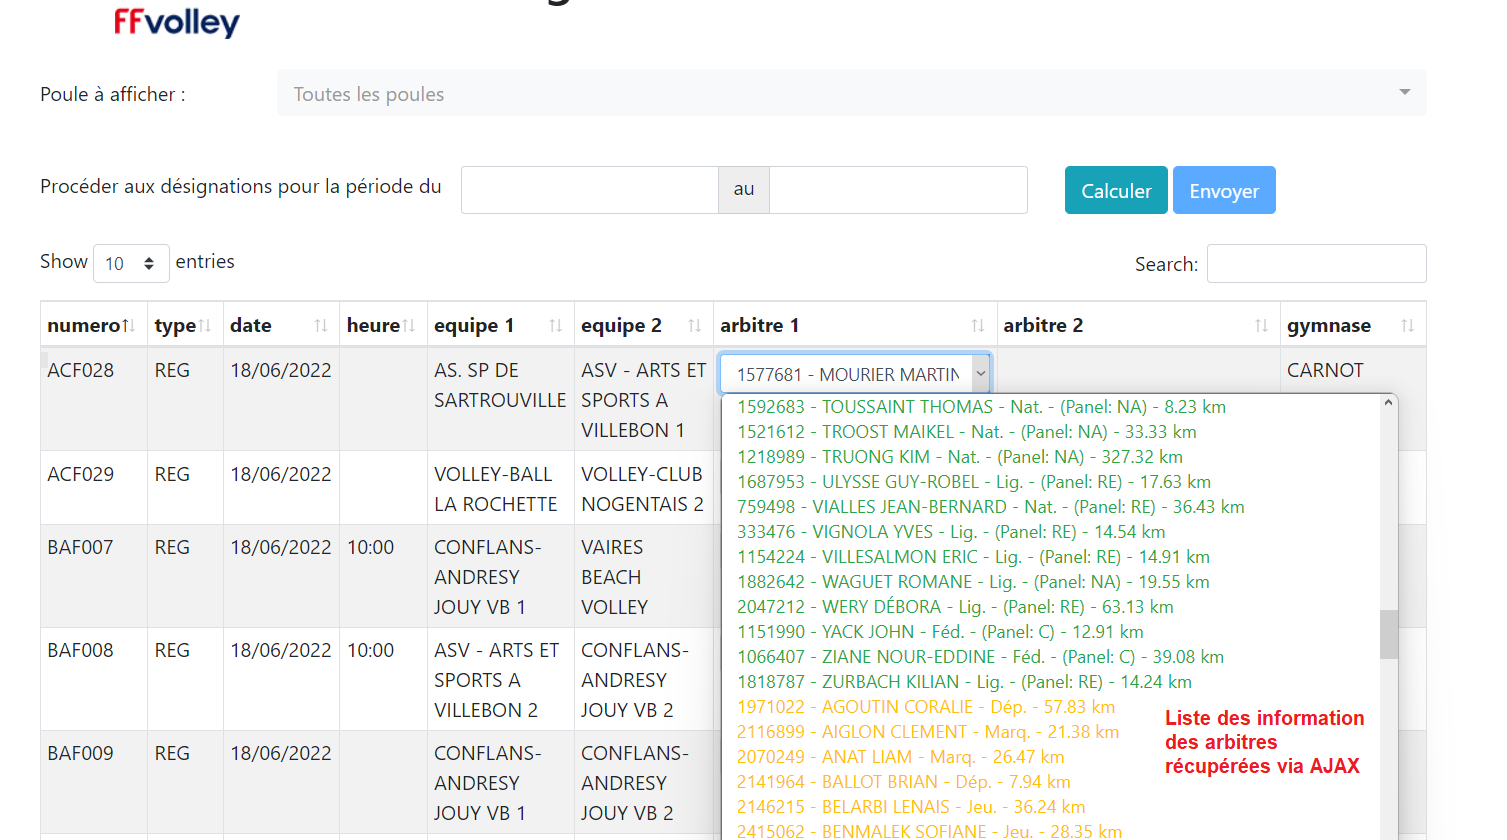
\includegraphics[width=\linewidth]{listedesg}
    \caption{Nouveau processus de désignation des arbitres}
\end{figure}

Pour faire ça, j’ai encore une fois utilisé JQuery pour envoyer une requête AJAX à une page qui récupère et me renvoi les bonnes informations d’arbitres pour le match voulu.

\begin{figure}[!h]
    \centering
    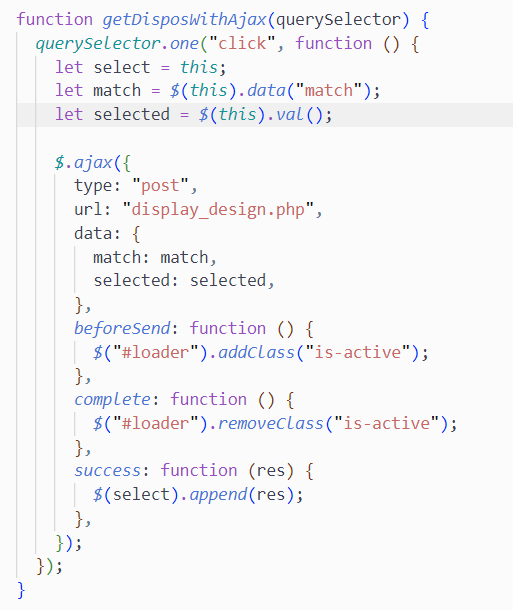
\includegraphics{getdispoajax}
    \caption{Fonction AJAX pour récupérer les arbitres}
\end{figure}

Cette façon de procéder a permis au chargement de la page de passer d’environ 180 secondes à moins de 2 secondes. Pour obtenir ces informations de performance, j’ai simplement affiché la différence en microsecondes entre la fin de mon script et le début.

\begin{figure}[!h]
    \centering
    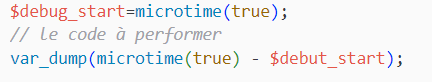
\includegraphics{debug}
\end{figure}

Au changement de sélection d’un arbitre pour le match, celui-ci est ensuite automatiquement intégré à la base de données grâce à l’envoi de ces informations via AJAX à une page annexe. Ceci permet alors d’éviter la perte de données  à un oubli.

\newpage 

\subsubsection{Désignations automatiques}
\vspace{1cm}

Pour rappel, l’algorithme de désignations automatique est construit de façon à prendre deux paramètres nullables qui correspondent aux date de la période pour laquelle effectuer ces désignations.\\ 

L’intégration de l’algorithme dans mon interface se fait donc simplement en envoyant ces valeurs via AJAX à une page annexe qui s’occupe de lancer l’algorithme et de renvoyer un tableau des matchs de la période avec les nouvelles désignations.
Ce tableau écrase ensuite celui déjà en place sur la page, et permet à son tour grâce aux fonctions Javascript de procéder aux désignations manuelles.

Les désignations automatiques doivent ensuite être validées grâce à un bouton, afin de les envoyer à une page qui s’occupe de les enregistrer dans la base de données.
\subsection{Sécurité}
\vspace{1cm}

Ce projet n’est qu’une branche d’une transition numérique plus importante, et est destiné à un public privé. Il n’a pour but d’être accessible que par les gestionnaires fédéraux grâce à des identifiants privés attribués par la fédération. \\

Le principal aspect de la sécurité pris en compte concerne les requêtes SQL car la base de données utilisée pour ce projet n’est pas directement liée à celle de la fédération. 
Ceci a été fait dans le cas d’un futur changement dans la récupération des paramètres pour effectuer ces requêtes. En effet, ces paramètres sont pour l’instant récupérés en interne mais pourraient potentiellement être récupérés par des formulaires.\\

De plus, les différentes pages permettant le renvoi d’informations via AJAX nettoient les données reçues grâce à la fonction \colored{htmlspecialchars()} pour éviter l’exploitation de la faille XSS. Cette faille permet à un attaquant d’envoyer du code malveillant sur un site, ce qui est contré par cette fonction car celle-ci transforme les balises html en entités correspondantes.\\

Finalement, aucun formulaire n’est intégré dans l’interface. Dans le cas contraire, il aurait fallut mettre en place un système de token pour éviter une exploitation malveillante de la faille CSRF. Ce système permet en effet de confirmer l’identité de la personne envoyant la requête.

\section{Documentation}
\vspace{1cm}

Afin de faciliter la reprise de cette partie par mon tuteur et mes successeurs, j’ai également écrit et mis en ligne une documentation complète. Celle-ci est écrite en Markdown (.md) et joue le rôle d’un cahier des spécifications techniques, permettant ainsi la compréhension du code en profondeur. 

\begin{figure}[!h]
    \centering
    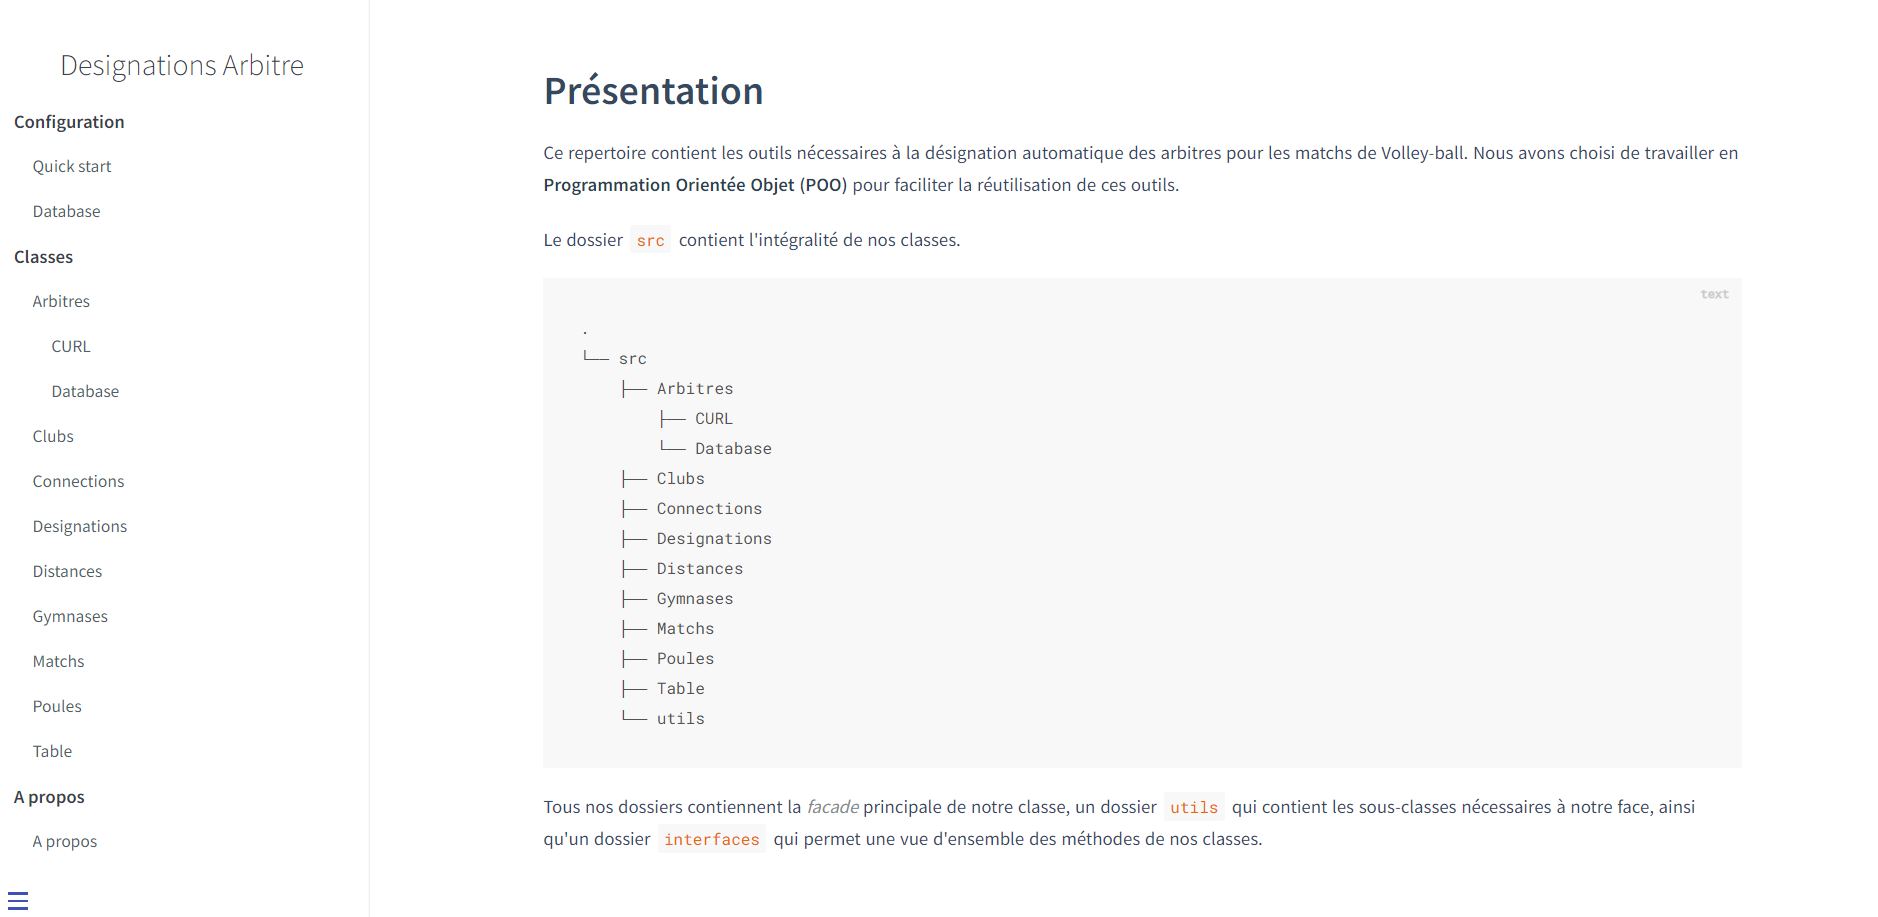
\includegraphics[width=\linewidth]{doc}
    \caption{Documentation en ligne pour le projet}
\end{figure}

La mise en page est gérée par \colored{Docsify}, une bibliothèque Javascript qui permet de convertir les fichiers markdown en pages HTML. Celle-ci permet ainsi de faciliter le rendu de la documentation, ce qui permet de se concentrer sur son contenu.\\

Pour la mise en ligne, j’ai opté pour le service gratuit de Google Firebase afin d’avoir une première intéraction avec cet outil.
\section{Conclusion}
\vspace{1cm}

Même si plusieurs points restent à améliorer, je suis satisfait de ce projet car toutes les demandes ont pu être mises en place. 
Celui-ci m’a permis de mettre en pratique les connaissances théoriques que j’avais pu acquérir en formation, mais également de prendre conscience d’aspects plus fonctionnels d’une application.\\

Devoir travailler sur une partie d’un projet plus grand m’a permis de me rendre compte de l’importance de la communication afin de mettre en place un plan de départ optimal, de l’importance de bien documenter son travail, ainsi que des avantages de découper son code pour une meilleure gestion du temps.

Il n’est pas toujours possible de savoir dans quelles conditions seront utilisés les outils que l’on met en place. Il faut donc pouvoir prendre en compte tous les aspects de ceux-ci

\end{document}